\documentclass[10pt]{beamer}
\usetheme{Singapore}
\usepackage{graphicx}
\usepackage{color}
\usepackage{mathptmx}
\usepackage{geometry}
\usepackage{multicol}
\usepackage{threeparttable}
\usepackage{cite}
\usepackage{tcolorbox}

\hypersetup{colorlinks,linkcolor=blue}

\setbeamertemplate{section in toc}[sections numbered] 
\setbeamertemplate{footline}[frame number]

\title[MPhil Thesis]{Import Exchange Rate Pass-Through and Credit Constraints: Evidence From China}
\author[Lingfei Lu]{\large Presenter: Lingfei Lu \\ \vspace{0.4cm} Supervisor: Prof. Yao Amber Li\\ \vspace{0.4cm} MPhil Thesis Defense \\ \vspace{0.4cm} Department of Economics}
\date{\today}
\logo{
\includegraphics[scale=0.15]{UST4C_L3.eps}}

\begin{document}
	
\begin{frame}[plain]
	\maketitle {}
\end{frame}

%----------------------------------------
\frame{
	\frametitle{Roadmap}
	\tableofcontents[] 
}

\setbeamertemplate{section in toc}[sections numbered] 
\setbeamertemplate{section in toc}[square] 

\section{Introduction}

\begin{frame}{Motivations}
	\begin{itemize}
		\item Exchange rate shock is a key factor affecting international trade price fluctuations.
		\item Exchange rate pass-through, the elasticity of local price changes to exchange rate fluctuations, measures how exchange rate risk is shared between buyers and sellers of trade.
		\item Understanding the pattern of exchange rate pass-through has important implications for formulating macro policy, including monetary policy, inflation targeting, and the balance of payments.
	\end{itemize}
\end{frame}

\begin{frame}{Motivations}
	\begin{itemize}
		\item The finance, macro and development literature emphasized that the variation in financial constraints across firms and industries could affect international trade as in \cite{manova2013}.
		\item It remains an open question whether importers under financial constraints will behave differently in price negotiation during exchange rate fluctuations.
		\item Therefore, we want to introduce industry-level credit constraints into the study of trade price elasticity with exchange rate shocks.
	\end{itemize}
\end{frame}

\begin{frame}{Key Questions}
Our research questions:
	\begin{itemize}
		\item [1] What is the difference in exchange rate pass-through (ERPT) patterns between Chinese importers and exporters?
		\item [2] How do credit constraints of importers affect import ERPT?
		\item [3] What are the channels through which credit constraints affect import ERPT? What factors would enhance or mitigate this effect?
	\end{itemize}
\end{frame}

\begin{frame}{What We Do}
Using Chinese customs transaction records, we find:	
	\begin{enumerate}
		\item The average import exchange rate pass-through level in China is significantly less complete than the export one.
		\item Tighter financial constraints will lead both import and export ERPT to be more complete.
		\item Importers with a wider sourcing base (who import a certain product from more sources) have a less complete ERPT and are less affected by credit constraints.
	\end{enumerate}	
\end{frame}

\section{Contribution}

\begin{frame}{Contribution to Literature: Incomplete Exchange Rate Pass-through}
	\begin{itemize}
		\item We first contribute to a wide literature on exchange rate disconnect, particularly on firm-level evidence of incomplete price pass-through.
		\item Two milestone papers link the exchange rate-price elasticity to
		disaggregated firm-level characteristics.
		\begin{itemize}
			\item \cite{bmm2012} (BMM) provide micro-level evidence of firm heterogeneity in response to real exchange rate shocks.
			\item \cite{aik2014} (AIK) find that
			firms with higher import intensity and larger market share have lower ERPT.
			\item Follow-ups: \cite{lmx2015}, \cite{chen2016}, \cite{garetto2016}, \cite{auer2016}, \cite{devereux2017}
		\end{itemize}
		\item Our contribution is to provides a novel perspective to study exchange rate disconnect in emerging markets, where firms are financially more vulnerable due to immature financial markets.
	\end{itemize}
\end{frame}

\begin{frame}{Contribution to Literature: Credit Constraints and Trade}
	\begin{itemize}
		\item Another important strand of literature discusses the effects of firms’ credit constraints on international trade: \cite{kroszner2007} \cite{manova2013}, \cite{chaney2016}, \cite {manova2013}, \cite{feenstra2015}, \cite{manova-wei-zhang2015}, \cite{fan-lai-li2015}.
		\item For the relationship between credit constraints and exchange rate pass-through, \cite{strasser2013} shows that financially constrained firms tend to pass more exchange rate shocks to prices.
		\begin{itemize}
			\item Two recent articles discussing credit constraints and ERPT with evidence from China, \cite{dai2021} and \cite{xu-guo2021}
		\end{itemize}
		\item We contribute to this literature by focusing on how importers behave under varying degrees of credit constraints and comparing their heterogeneous capacity to absorb exchange rate shocks. 
	\end{itemize}	
\end{frame}

\section{Data}

\begin{frame}{Data: Customs Transaction Records}
	\begin{itemize}
		\item The first dataset is the transaction level records from the General Administration of Customs of China (GACC) during 2000-2011.
		\begin{itemize}
			\item This dataset provides information on
			all Chinese trade transactions including import and export values, quantities, units, product names and codes, source and destination countries, and type of enterprises.
			\item The categories of products are coded by the Harmonized Coding and Description System (HS) from World Customs Organization (WCO).
		\end{itemize}
		\item We drop unwanted observations referring to \cite{lmx2015}:
		\begin{itemize}
			\item products with inconsistent missing information of unit or quantity
			\item special product categories such as arms (HS2=93), antiques (HS2=97), and special categories (HS2=98 and 99)
			\item transactions existing for only one year without any change over time.
		\end{itemize}
	\end{itemize}
\end{frame}

\begin{frame}{Data: Firm-level Information}
	\begin{itemize}
		\item The second dataset is Chinese Industrial Enterprises (CIE) database from the National Bureau of Statistics of China (NBSC).
		\begin{itemize}
			\item This dataset covers all state-owned enterprises and above-scale firms
			with annual sales of more than 5 million RMB from 1999 to 2007.
			\item The data provide details about firms’ identification code, ownership, industry
			type, and about 80 other variables in the balance sheet including the number of employees, total wage payments, the value of fixed assets, sales income, total operation inputs, etc.
		\end{itemize}
		\item To merge it with customs records, we match the identification codes based on the contact information of firms as in \cite{fan-li-yeaple2015}.
	\end{itemize}
\end{frame}

\begin{frame}{Data: Summary Statistics}
	\begin{itemize}
		\item The summary statistics of the whole customs records, the firm information dataset, and the final matched sample are shown in the panels A, B, and C below, respectively:
	\end{itemize}
	\begin{figure}[htbp]
		\centering
		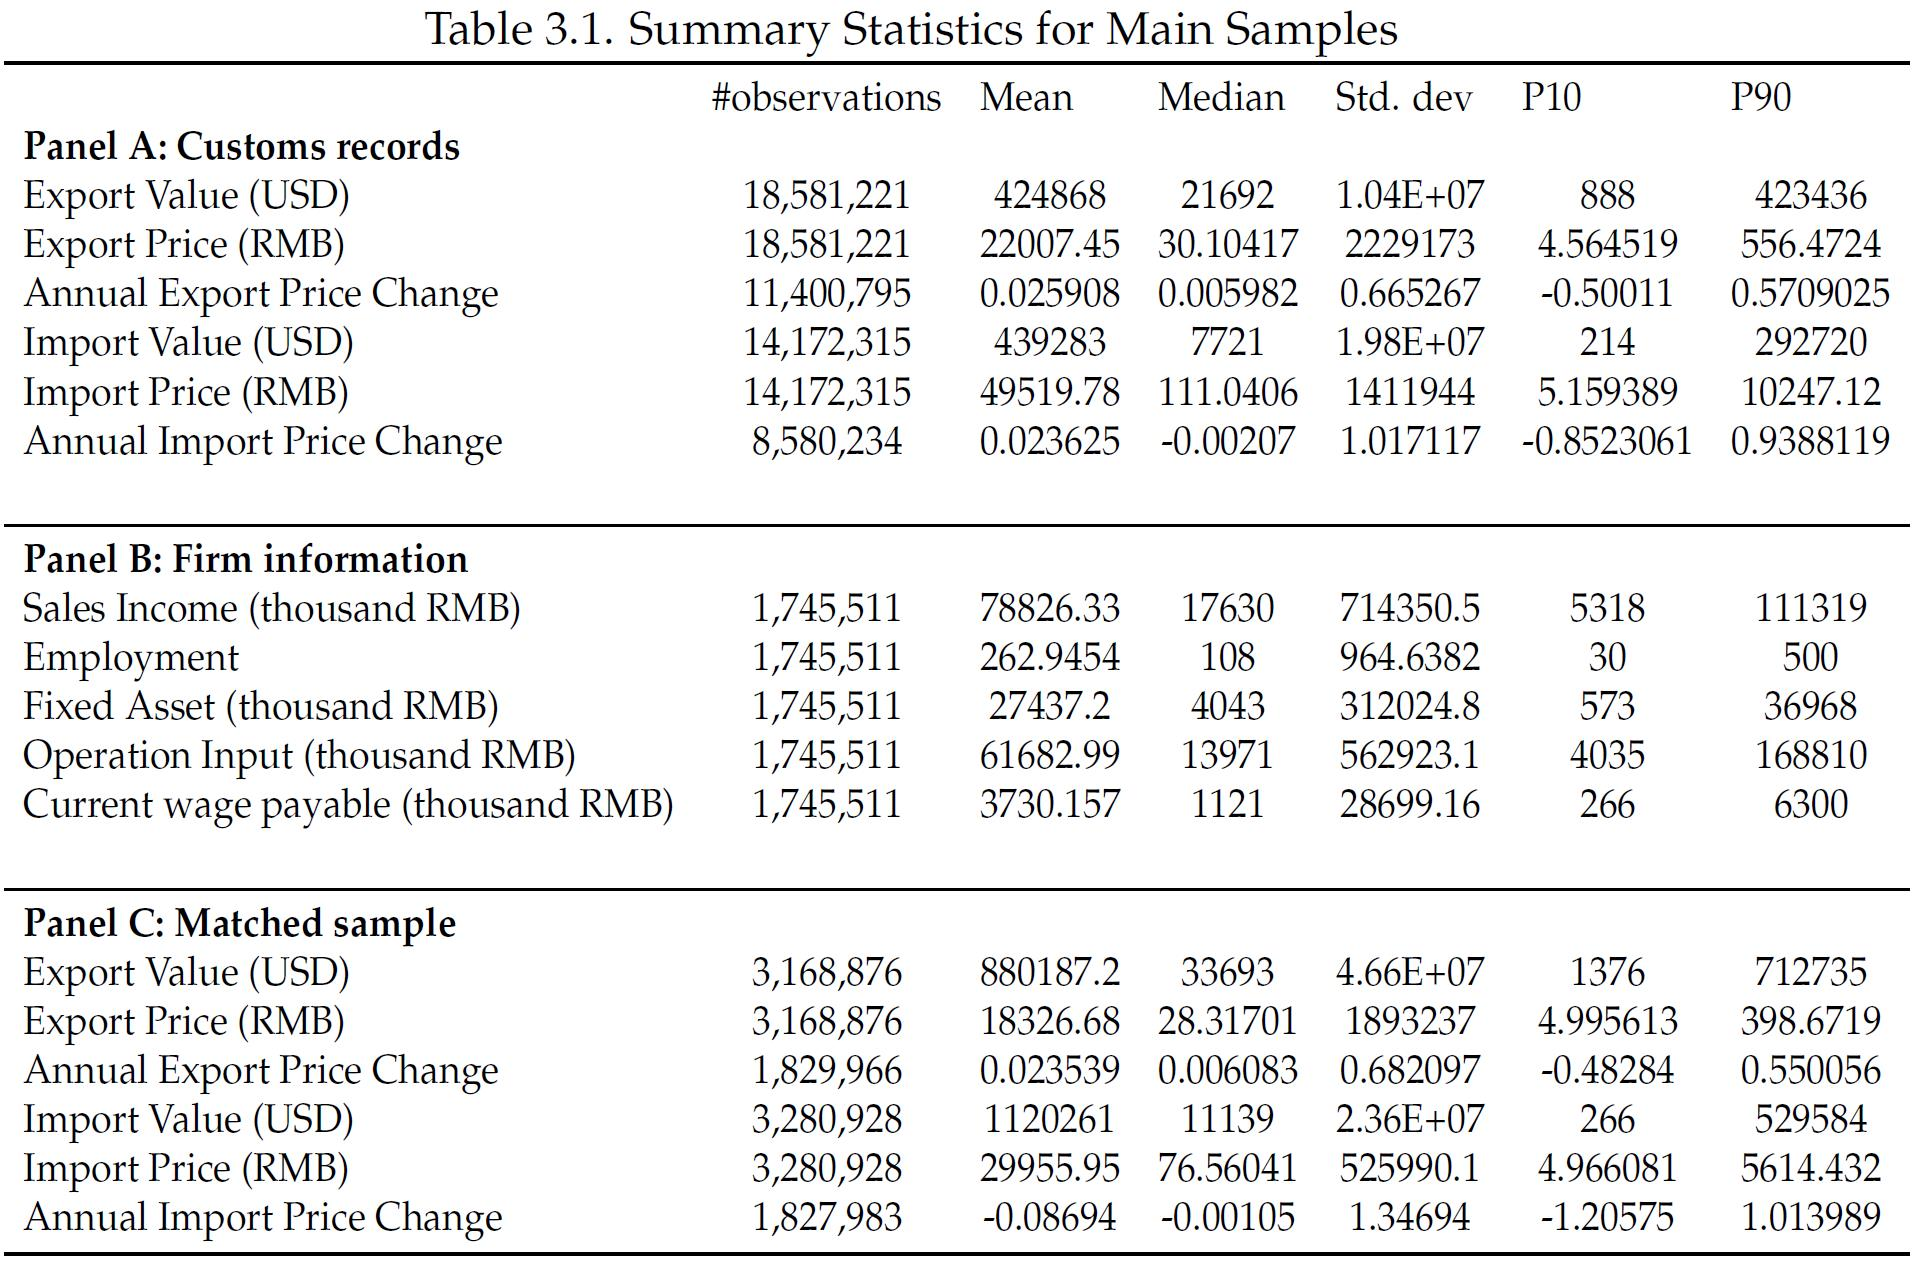
\includegraphics[height=0.65\textheight]{Table3.1.jpg}
		\label{tab3.1}
	\end{figure}
\end{frame}

\begin{frame}{Data: Exchange Rates and Macro Variables}
	\begin{itemize}
		\item Nominal exchange rates and price level of household consumption are from Penn World Table (PWT) 10.0 \cite{feenstra2015}.
		\item The bilateral nominal exchange rate is defined as the number of home currency units that can purchase a unit of foreign currency.
		\item The CPI-based real exchange rate ($RER_{ct}$) is defined as:
		$$
		RER_{ct}=NER_{ct} \cdot \frac{CPI_{ct}}{CPI_{CHN,t}}.
		$$
		\item An increase in $RER_{ct}$ means a real depreciation of the Chinese RMB against the
		foreign country’s $c$ currency.
		\item In addition, we use the real GDP of the destination countries from PWT 10.0, computed with national-accounts growth, $RGDP_{ct}$.
	\end{itemize}
\end{frame}

\begin{frame}{Data: Exchange Rates Fluctuations}
	\begin{itemize}
		\item We saw substantial variations in RMB exchange rate fluctuations against major trading partners of China during 1999-2011.
		\begin{columns}
			\column{0.5\columnwidth}
			\begin{figure}[htbp]
				\centering
				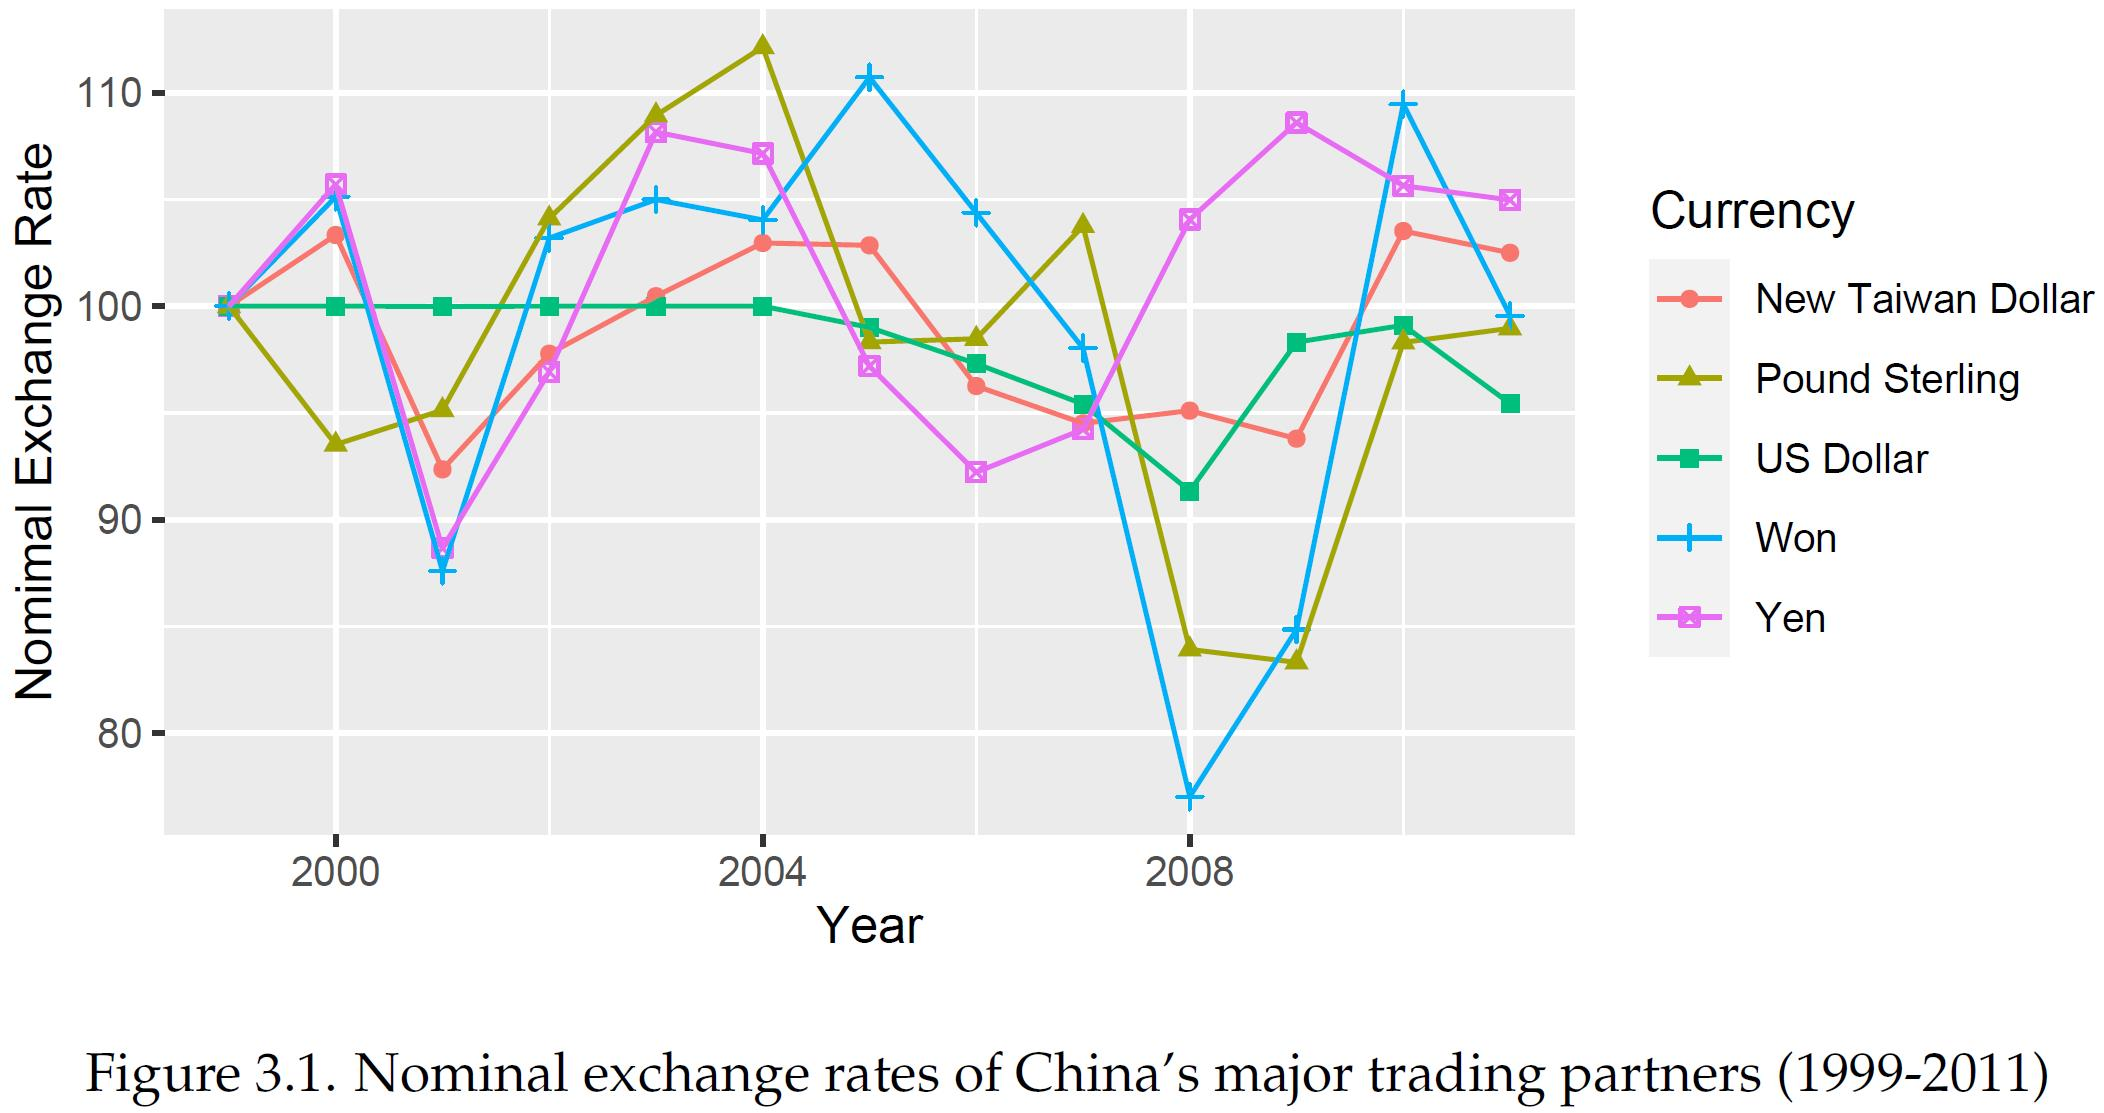
\includegraphics[width=1.1\columnwidth]{Figure3.1.jpg}
				\label{fig3.1}
			\end{figure}
			\column{0.5\columnwidth}
			\begin{figure}[htbp]
				\centering
				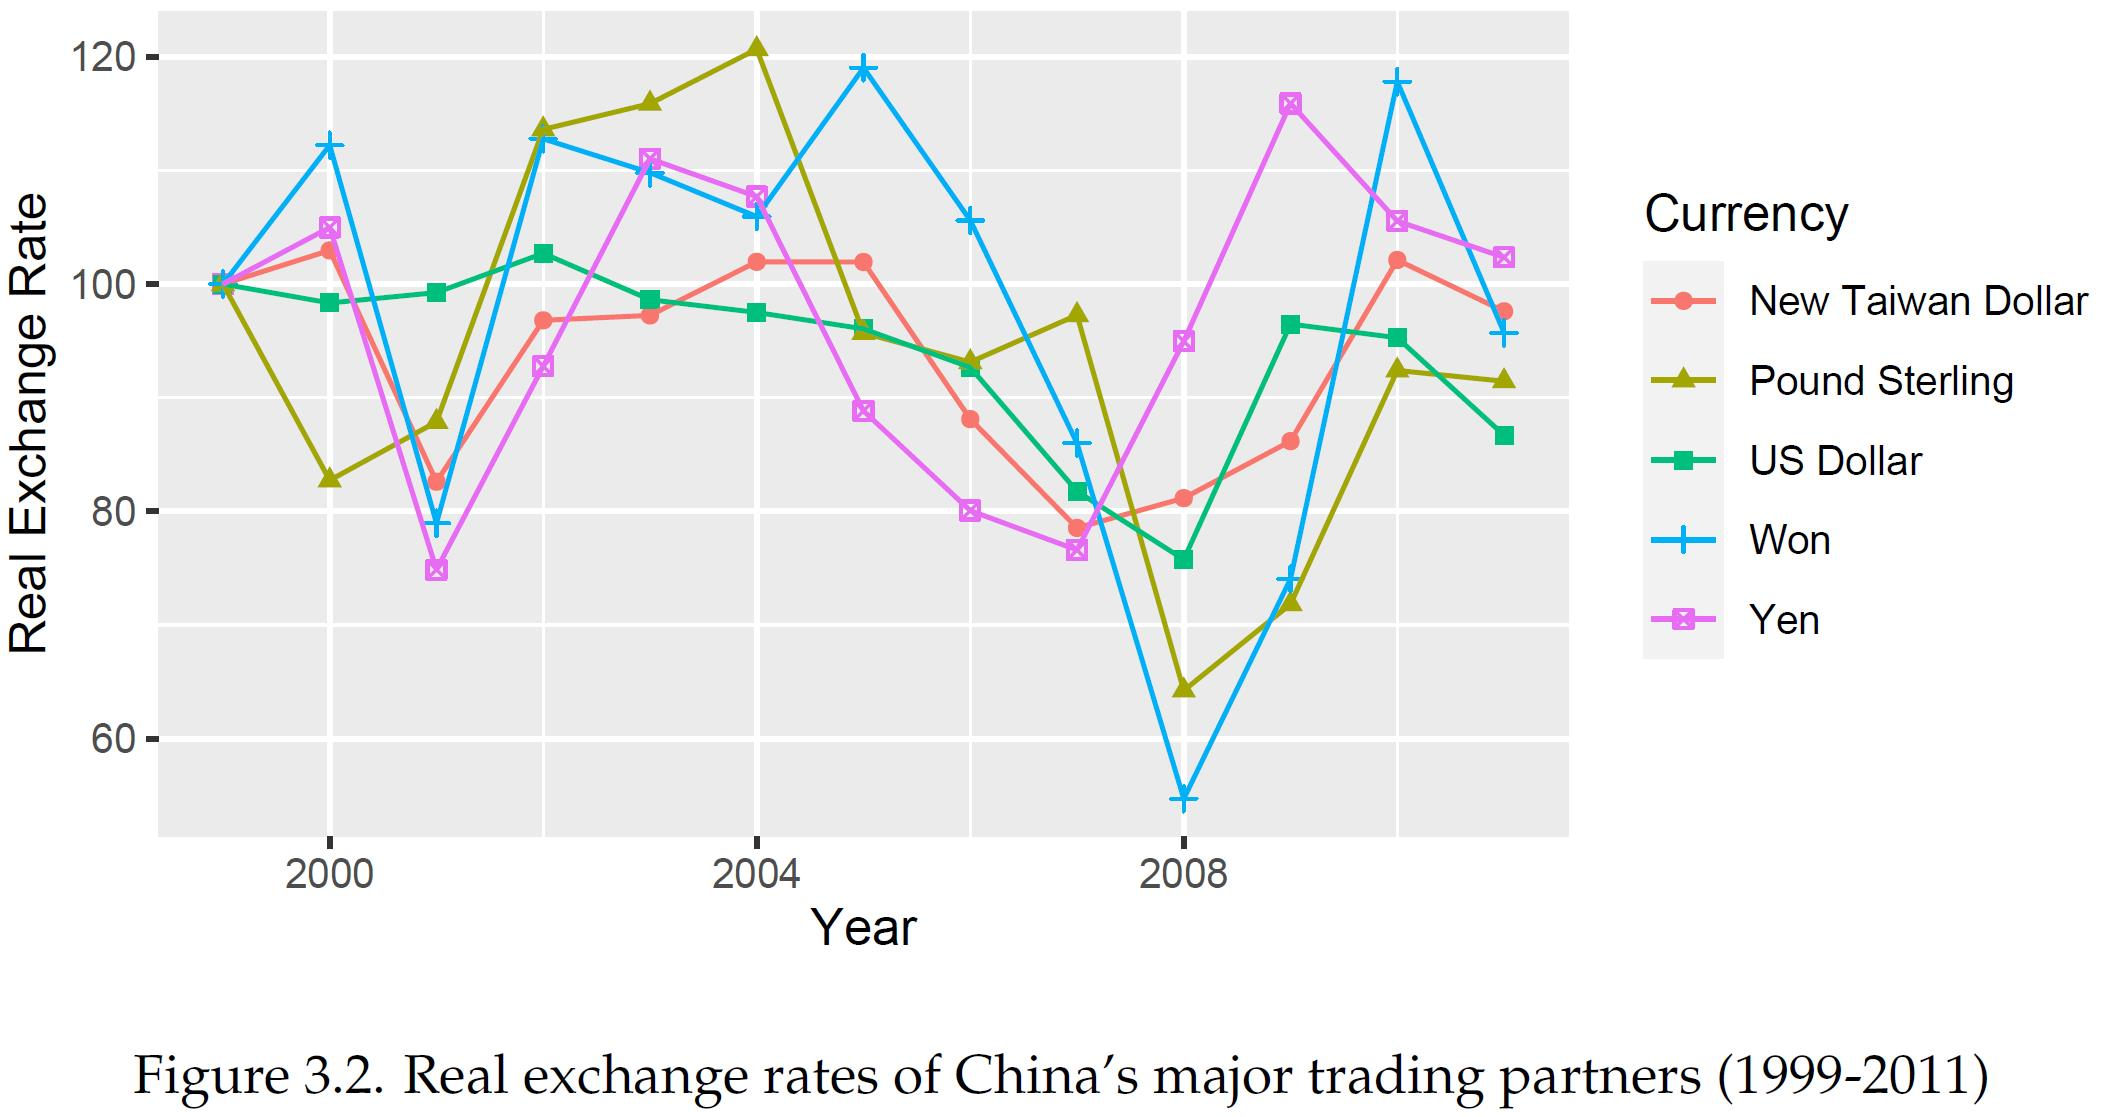
\includegraphics[width=1.1\columnwidth]{Figure3.2.jpg}
				\label{fig3.2}
			\end{figure}
		\end{columns}
		\item The real exchange rate against the US dollar did not change a lot in 2000-2004 due to the nominal pegging scheme. In 2005, the peg was lifted to appreciation due to the evolution of exchange policy.
	\end{itemize}
\end{frame}

\section{Empirical Framework}

\begin{frame}{Baseline Estimation Equation}
	\begin{itemize}
		\item The first step goal is to estimate exchange rate pass-through as the elasticity of unit values changes to exchange rate changes.
		\begin{equation}
			\Delta \ln P^{D}_{i j c t}=\alpha+\beta^D \Delta \ln R E R_{c t}+\gamma \Delta \ln R G D P_{c t}+\xi_{i j c}+\tau_{t}+\varepsilon_{i j c t}
			\label{eq4.1}
		\end{equation}
		{\footnotesize where $P_{ijct}$ is the price of the product $i$ bought (sold) by firm $j$ from country $c$ in year $t$.  $D \in$ \{Import, Export\} denotes the trade direction. $\xi_{ijc}$ denotes the firm-product-country level fixed effects. $\tau_t$, the year dummies, control for common macro-shocks across firms.}
		\item To deal with possible non-stationarity, we use the first difference of the logarithms for prices $\Delta \ln P^{D}_{i j c t}$, real exchange rates $\Delta \ln R E R_{c t}$ and real GDP $\Delta \ln R G D P_{c t}$ to represent their annual rates of change.
	\end{itemize}
\end{frame}

\begin{frame}{Unit Value as Price}
	\begin{itemize}
		\item The customs records contain trade values (by US dollars) and quantities for each HS6 product $i$, each firm $j$, from (or to) each country $c$, in each year $t$, $V_{ijct}$, and $Q_{ijct}$.
		\item The real prices for export and import $P^{Import}_{i j c t}$ and $P^{Export}_{i j c t}$ are computed as unit values, both denominated by the Chinese RMB:
		$$
		P^{D}_{ijct}=\frac{V^{D}_{ijct}\cdot NER_{US,t}}{Q^{D}_{ijct}}
		$$
		\item Because product categories are highly subdivided, we believe that the unit value is an ideal proxy for the transaction price.
	\end{itemize}
\end{frame}

\begin{frame}{Baseline Estimation Coefficients}
	\begin{itemize}
		\item The coefficient $\beta^{D=Import}$ measures the completeness of import exchange rate pass-through, i.e. a higher $\beta$ means Chinese importers face more volatile import RMB prices during exchange rate shocks.
		\item However,  $\beta^{D=Export}$ means the "incompleteness" of the export pass-through because a higher $\beta$ means Chinese exporters pass less exchange rate change to the destination market while having more volatile domestic currency prices.
	\end{itemize}
\end{frame}

\begin{frame}{Estimations with Credit Constraints}
	\begin{itemize}
		\item We study the credit constraint effects on exchange rate pass-through by including an interaction term of sectors’ financial vulnerability:
		\begin{equation}
			\begin{aligned}
				\Delta \ln P^{D}_{ijct}=&\alpha+\beta^D_{1} \Delta \ln RER_{ct}+\beta^D_{2} \Delta \ln RER_{ct} \cdot FV_{j} \\ &+\gamma \Delta \ln RGDP_{ct}+\xi_{ijc}+\tau_{t} +\varepsilon_{ijct}
			\end{aligned}
			\label{eq4.2}
		\end{equation}
		{\footnotesize where $FV_{j}$ is the financial vulnerability of the sector to which the firm $j$ belongs.}
		\item The interaction coefficient $\beta_2$ represents the effect of industry-level credit constraints on exchange rate pass-through.
		\item The overall import ERPT for firm $j$ is given by $\beta^D_{1} +\beta^{Import}_{2} FV_j$ and the overall export ERPT is $\beta^D_{1} +\beta^{Export}_{2} FV_j$.
	\end{itemize}
\end{frame}

\begin{frame}{Measures of Credit Constraints}
	\begin{itemize}
		\item Following \cite{manova-wei-zhang2015} and \cite{fan-lai-li2015}, we use sector-level financial vulnerability measures to proxy for credit needs (demand for outside capital) and the ability to resist financial risks.
		\begin{enumerate}
			\item \textbf{External Finance Dependence ($ExtFin_j$)}: the share of capital expenditures not financed by operational cash flows.
			\item \textbf{Asset Tangibility ($Tang_j$)}: the share of the net value of tangible assets that firms can pledge as collateral to raise external finance, in its total book value.
			\item \textbf{Inventory-to-sales Ratio ($Invent_j$)}: measure of the production cycle duration and the necessary working capital to maintain inventories and meet demand. 
		\end{enumerate}
		\item We also construct the \textbf{first principal component} $FPC_j$ of external finance dependence and asset tangibility as an aggregate measure.
	\end{itemize}
\end{frame}

\begin{frame}{Measures of Credit Constraints}
	\begin{itemize}
		\item Alternatively, we also compute measures of credit needs based on Chinese firm-level information, with an additional of R\&D intensity.
		\item Below are the summary statistics of US and Chinese measures of credit constraints.
		\begin{figure}[htbp]
			\centering
			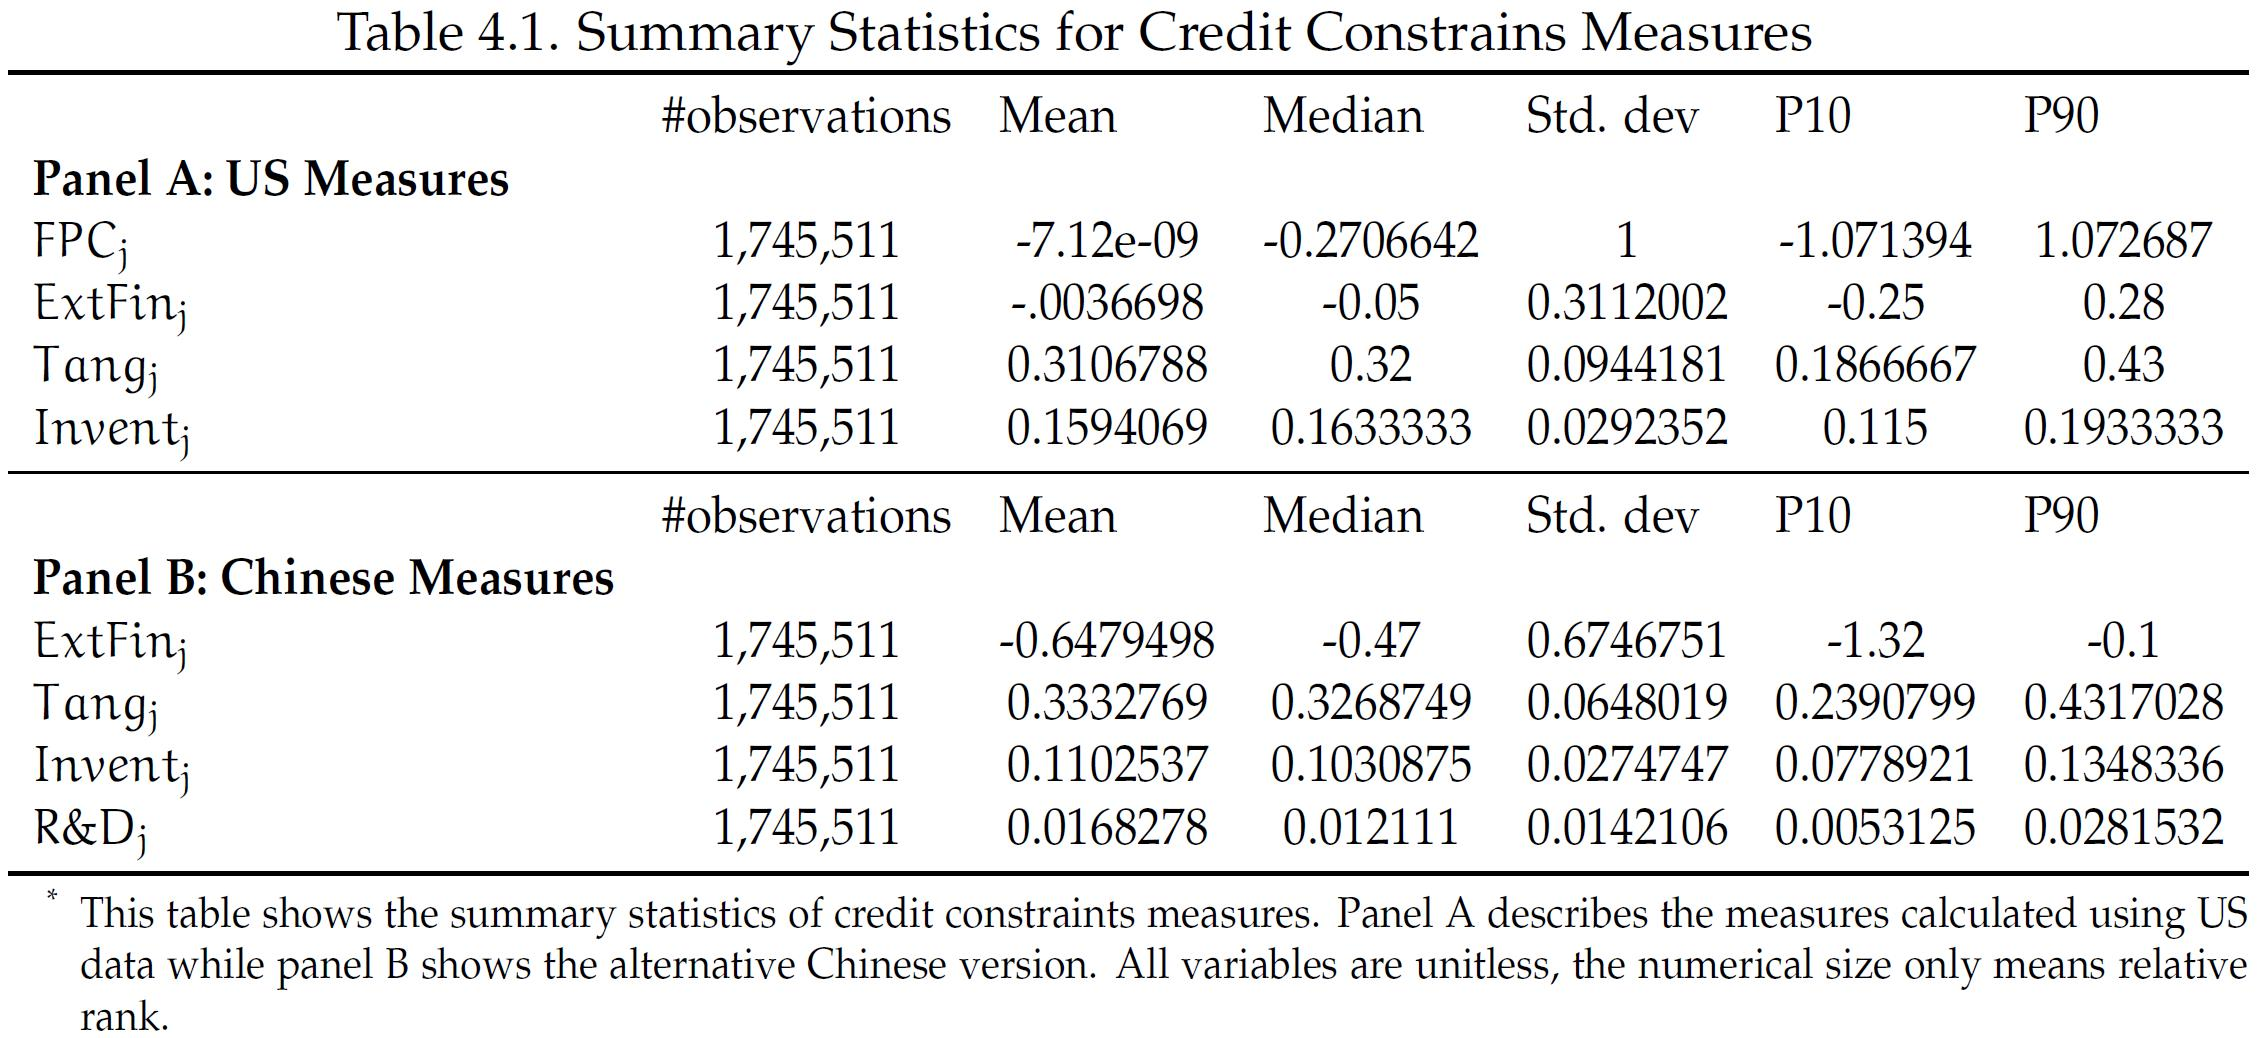
\includegraphics[width=0.9\textwidth]{Table4.1.jpg}
			\label{tab4.1}
		\end{figure}
	\end{itemize}
\end{frame}

\begin{frame}{Additional Firm-level Factors}
	To answer the third question, we introduce a vector $\mathbb{Z}_{jt}$ (or its lagged form $\mathbb{Z}_{jt-1}$) to include additional factors which may affect ERPT.
	\begin{enumerate}
		\item \textbf{Sourcing Diversity}: defined as the number of source countries from which an importer $j$ imports a certain HS6 product type $i$. 
		\item \textbf{Markup}: estimated by the GMM method following \cite{dlw2012} and \cite{bkl2021}.
		\item \textbf{Market Share}: defined as a firm’s value share in the import market, within a given HS6 product category.
		$$
		S^{D}_{ijct} \equiv \frac{v^{D}_{ijct}}{\sum_{j^{\prime} \in J_{ict}} v^{D}_{ij^{\prime}ct}}
		$$
	\end{enumerate}
\end{frame}

\begin{frame}{Estimations with Additional Factors}
	\begin{itemize}
		\item Estimation equations with additional factors $\mathbb{Z}_{jt-1}$:
		\begin{equation}
			\begin{aligned}
				\Delta \ln P^{D}_{ijct} =&\alpha+[\beta^D_{1}+ \beta^D_{2} \cdot FV_{j}+\beta^D_{3} \cdot {\mathbb{Z}^{D}_{jt-1}}'] \Delta \ln RER_{ct} \\
				&+\gamma \Delta \ln RGDP_{ct}+ {\mathbb{Z}^{D}_{jt}}' \eta+\xi_{ijc}+\tau_{t} +\varepsilon_{ijct}.
				\label{eq4.3}
			\end{aligned}	
		\end{equation}
		
		\begin{equation}
			\begin{aligned}
				\Delta \ln P^{D}_{ijct}=&\alpha+[\beta^D_{1}+ \beta^D_{2} \cdot FV_{j}+\beta^D_{3} \cdot {\mathbb{Z}^{D}_{jt-1}}'+\beta^D_{4} \cdot FV_{j} \cdot {\mathbb{Z}^{D}_{jt-1}}'] \Delta \ln RER_{ct} \\ 
				&+\gamma \Delta \ln RGDP_{ct}+ {\mathbb{Z}^{D}_{jt}}' \eta+\xi_{ijc}+\tau_{t} +\varepsilon_{ijct}.
			\end{aligned}	
			\label{eq4.4}
		\end{equation}
		\item When using market share and its square term as additional factors:
		\begin{equation}
			\begin{aligned}
				\Delta \ln P^{D}_{ijct}=&\alpha+[\beta^D_{1}+ \beta^D_{2} \cdot FV_{j}+\beta^D_{3} \cdot S^{D}_{ijct}+\beta^D_4 \cdot {S^{D}_{ijct}}^2] \Delta \ln RER_{ct} \\
				&+\gamma \Delta \ln RGDP_{ct}+ \eta S^{D}_{ijct}+\xi_{ijc}+\tau_{t} +\varepsilon_{ijct}.
			\end{aligned}
			\label{eq4.5}
		\end{equation}
	\end{itemize}
\end{frame}

\section{Main Results}

\begin{frame}{Results: Import Pass-through vs Export Pass-through}
	\begin{itemize}
		\item The results for import exchange rate pass-through versus export exchange rate pass-through are shown below using different samples.
	\end{itemize}
	\begin{figure}[htbp]
		\centering
		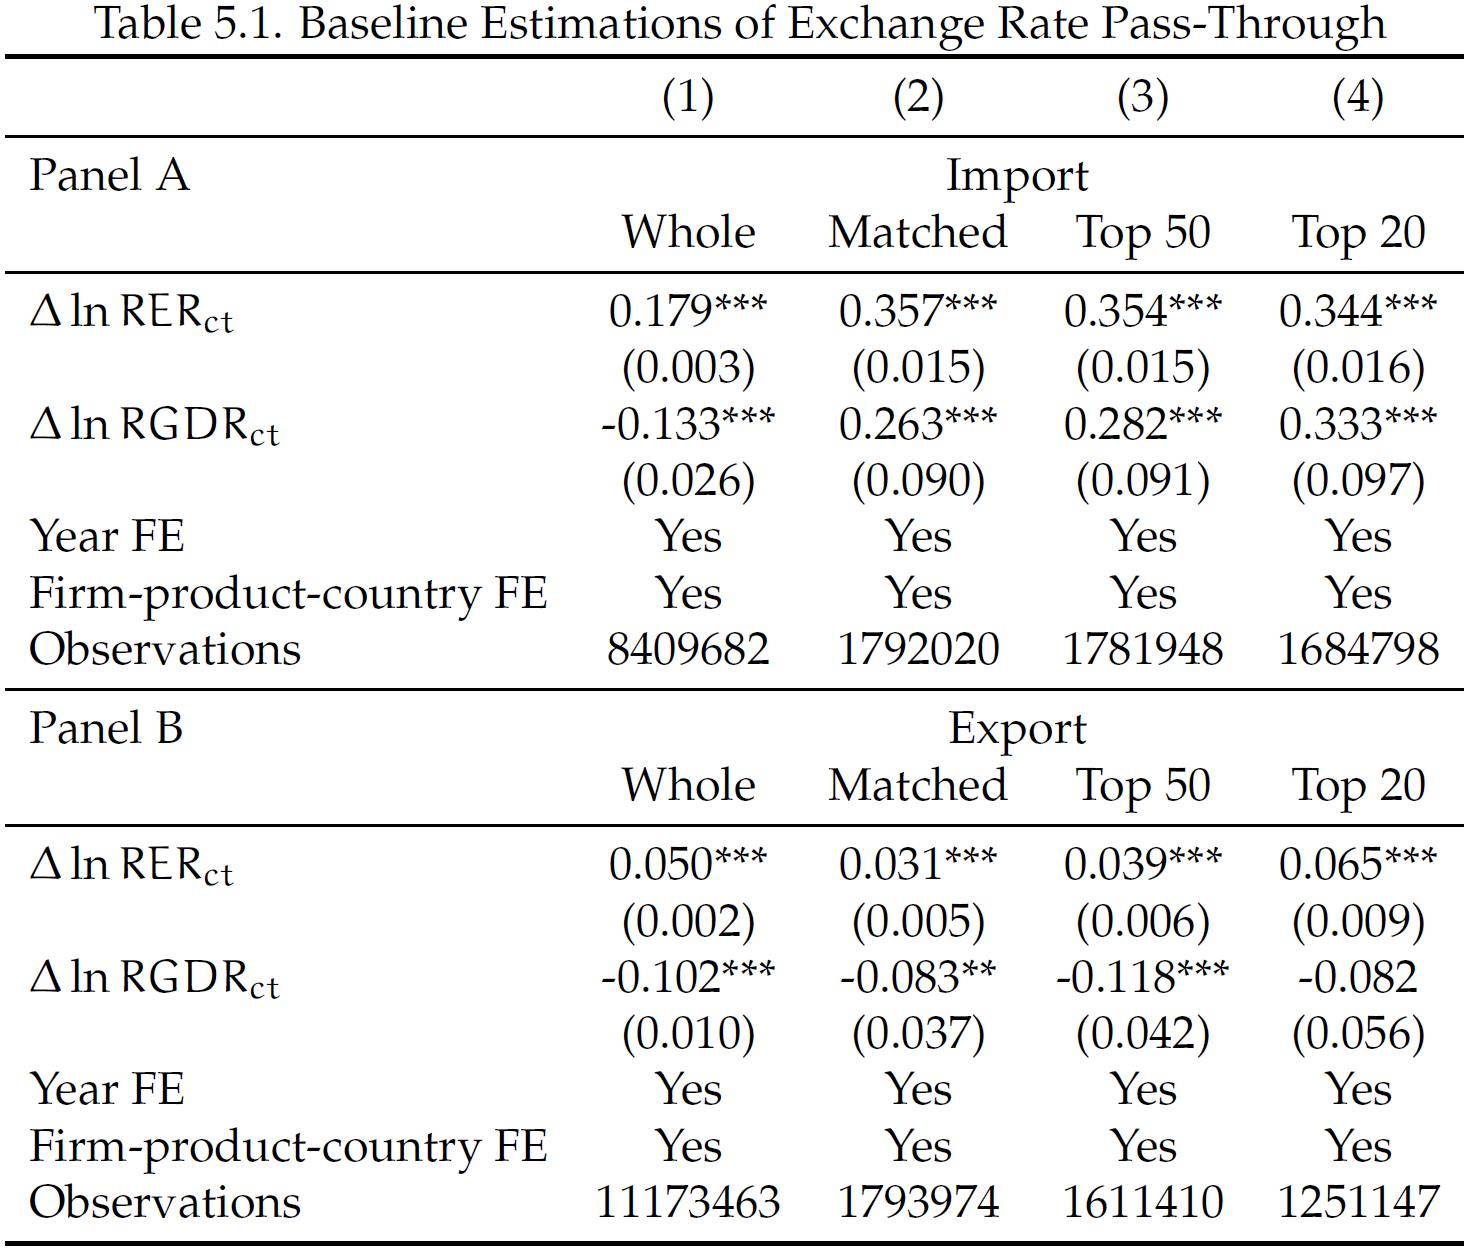
\includegraphics[width=0.7\columnwidth]{Table5.1.jpg}
		\label{tab5.1}
	\end{figure}
\end{frame}

\begin{frame}{Results: Import Pass-through vs Export Pass-through}
	\begin{tcolorbox}[colback=blue!5!white, colframe=blue!75!black,title=Key Finding 1]
		\begin{itemize}
			\item The average import exchange rate pass-through level in China is significantly less complete than the export one.
		\end{itemize}
	\end{tcolorbox}
	\begin{itemize}
		\item For Chinese firms, when RMB depreciates against the currencies of major trading partners, export prices denominated in RMB will not rise significantly, but their import costs will rise more; 
		\item When RMB appreciates, export prices in RMB will decrease only to a limited extent, and their import costs will drop more.
	\end{itemize}
\end{frame}

\begin{frame}{Results: Effects of Credit Constraints}
	\begin{itemize}
		\item Panel A presents differences in import exchange rate pass-through caused by industry-level credit demand heterogeneity as equation \ref{eq4.2}.
	\end{itemize}
	\begin{figure}[htbp]
		\centering
		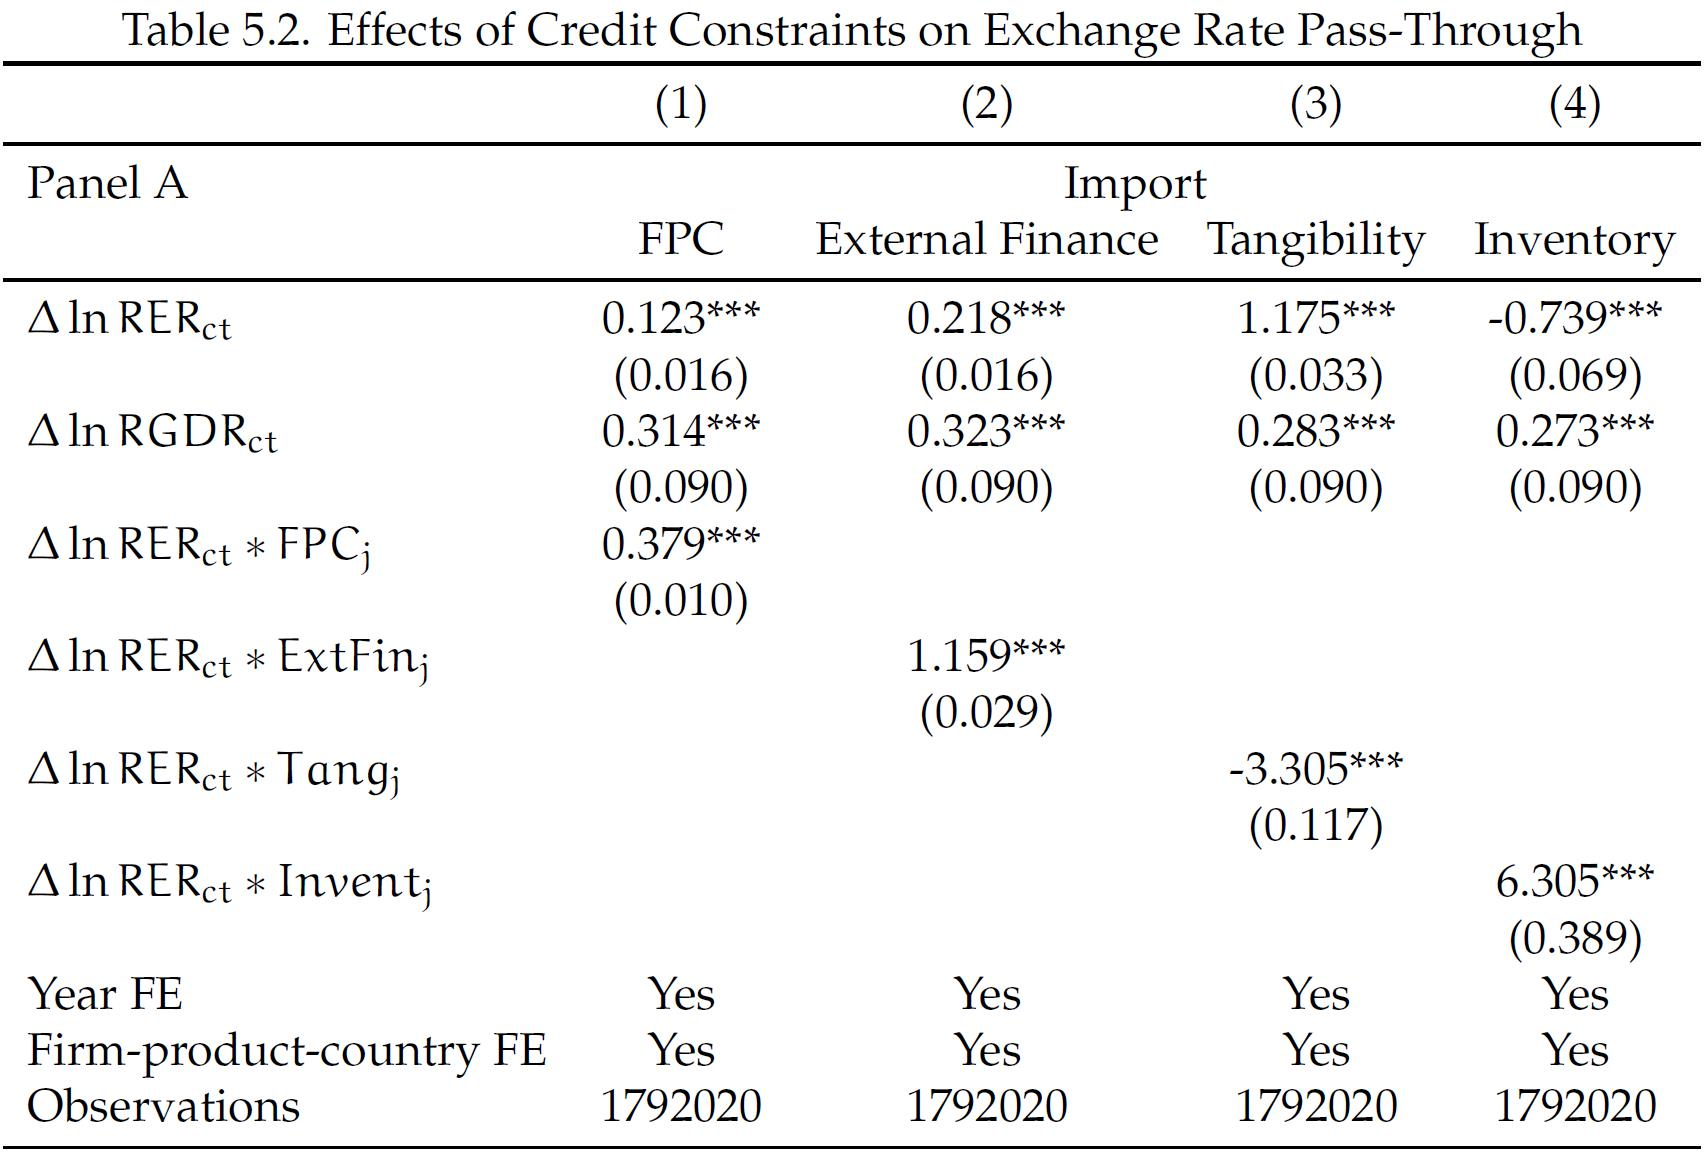
\includegraphics[width=0.8\columnwidth]{Table5.2A.jpg}
		\label{tab5.2A}
	\end{figure}
\end{frame}

\begin{frame}{Results: Effects of Credit Constraints}
	\begin{itemize}
		\item Panel B presents comparable results for effects of credit constraints on export exchange rate pass-through.
	\end{itemize}
	\begin{figure}[htbp]
		\centering
		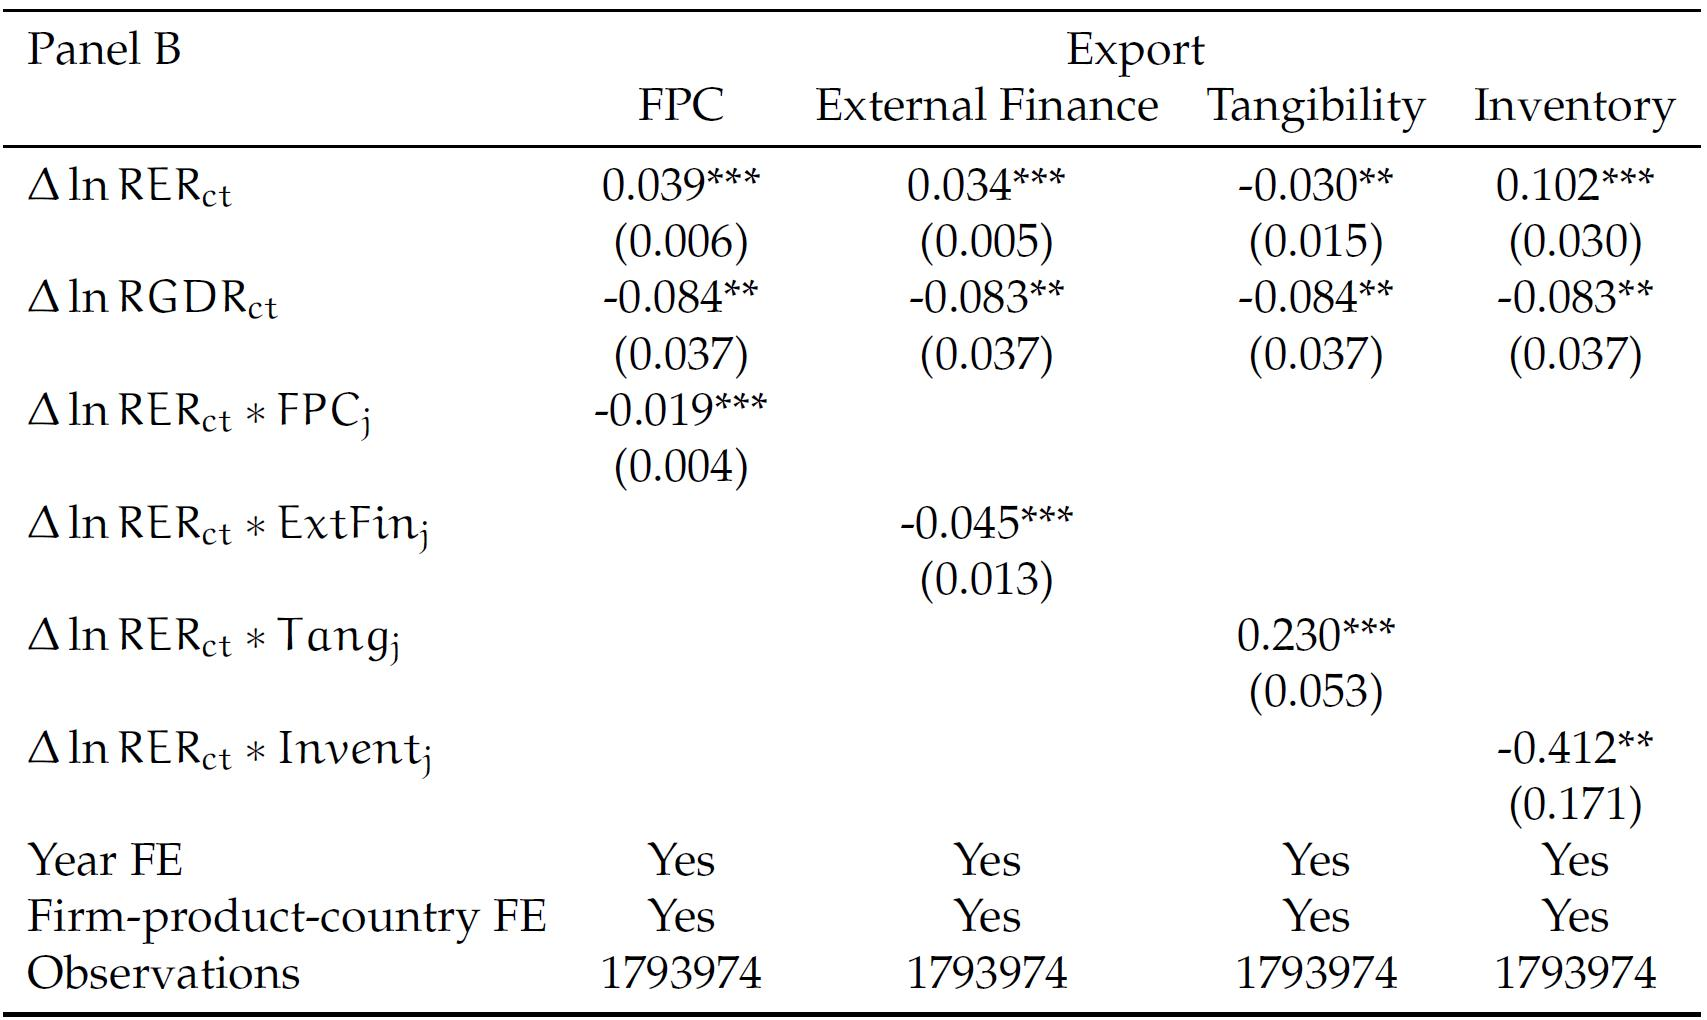
\includegraphics[width=0.8\columnwidth]{Table5.2B.jpg}
		\label{tab5.2B}
	\end{figure}
\end{frame}

\begin{frame}{Results: Effects of Credit Constraints}
	\begin{tcolorbox}[colback=blue!5!white, colframe=blue!75!black,title=Key Finding 2]
		\begin{itemize}
			\item Tighter financial constraints will lead both import and export ERPT to be more complete.
		\end{itemize}
	\end{tcolorbox}
	\begin{itemize}
		\item \textit{Credit constraints expose Chinese manufacturing firms to greater exchange rate risk in international trade.}
		\item Exporters with more vulnerable credit lower destination prices more when RMB depreciates, while RMB revenue remained stable, and restricted importers' costs rose more significantly; 
		\item When RMB appreciates, restricted exporters will increase destination prices more, even if it means losing their competitive advantages, and restricted importers' costs will be reduced.
	\end{itemize}
\end{frame}

\begin{frame}{Results: Sourcing Diversity and Credit Constraints}
	\begin{figure}[htbp]
		\centering
		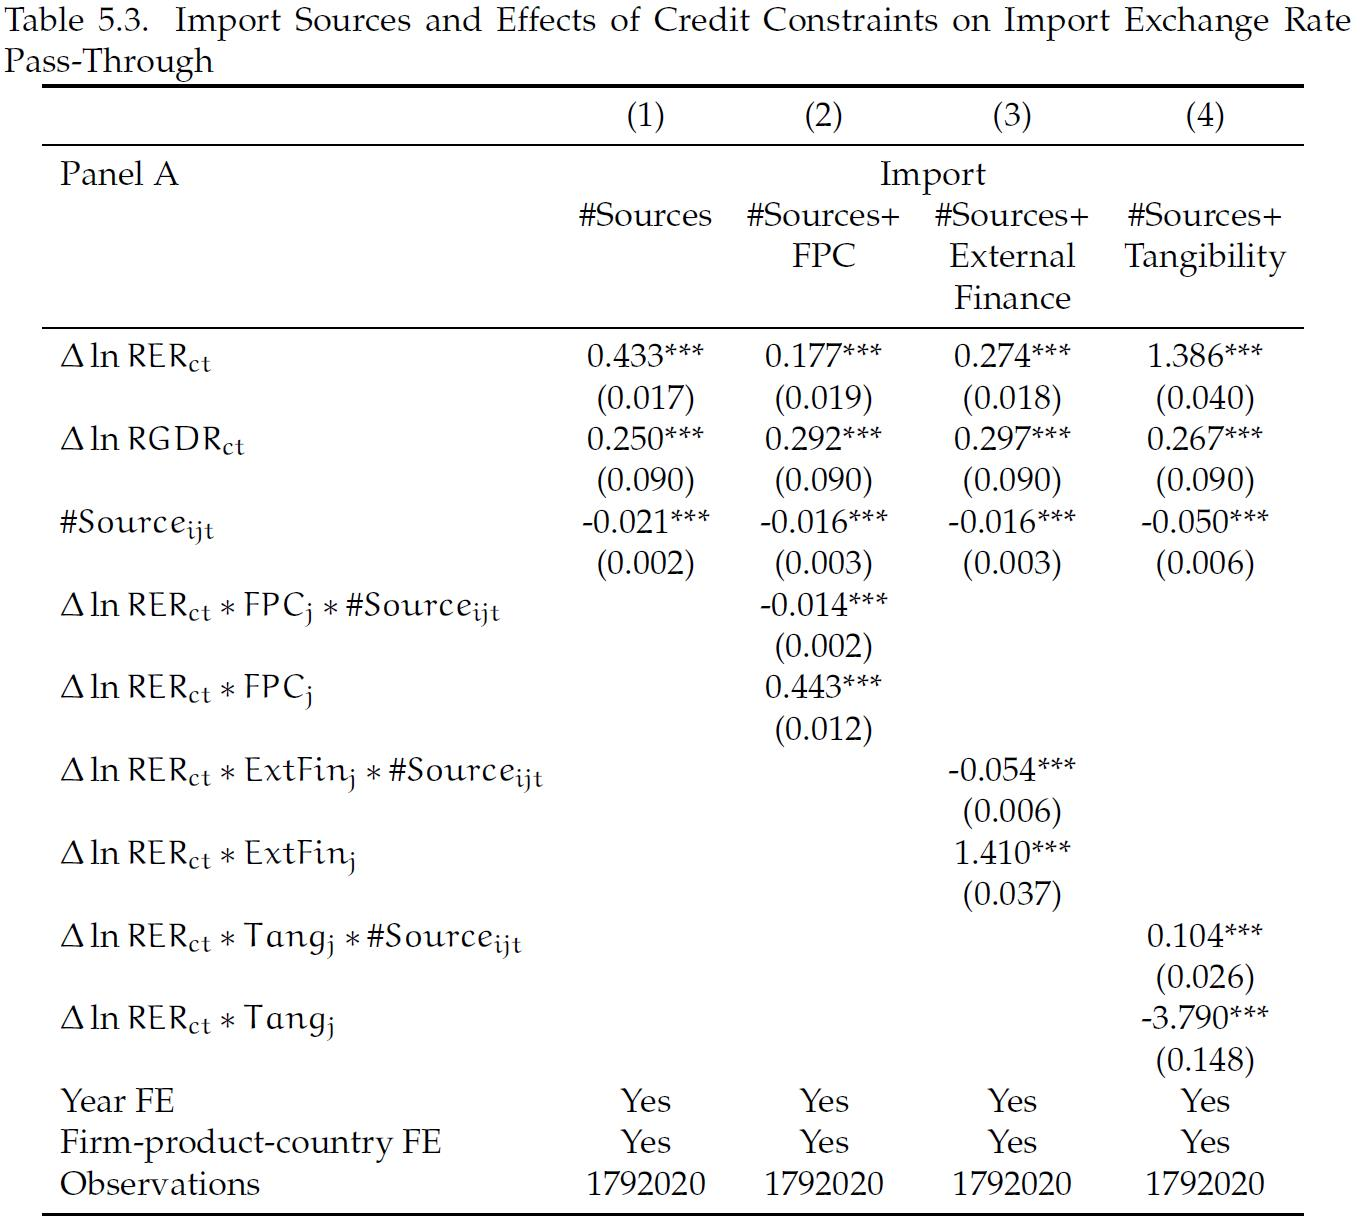
\includegraphics[width=0.75\columnwidth]{Table5.3.jpg}
		\label{tab5.3}
	\end{figure}
\end{frame}

\begin{frame}{Results: Sourcing Diversity and Credit Constraints}
	\begin{tcolorbox}[colback=blue!5!white, colframe=blue!75!black,title=Key Finding 3]
		\begin{itemize}
			\item Importers with a wider sourcing base (who import a certain product from more sources) have a less complete ERPT and are less affected by credit constraints.
		\end{itemize}
	\end{tcolorbox}
	\begin{itemize}
		\item If a firm can import the same product from more sources, it has more flexibility to escape the unfavorable exchange rate risk.
		\item A more diverse importer can either switch from one source to another to reduce costs (trade diversion effect), or make a more credible threat to negotiate a more stable price.
	\end{itemize}
\end{frame}

\section{Robustness}

\begin{frame}{Alternative Measures of Credit Constraints}
	\begin{itemize}
		\item Robustness check test 1: we use alternative credit constraint measures constructed from Chinese data.
	\end{itemize}
	\begin{figure}[htbp]
		\centering
		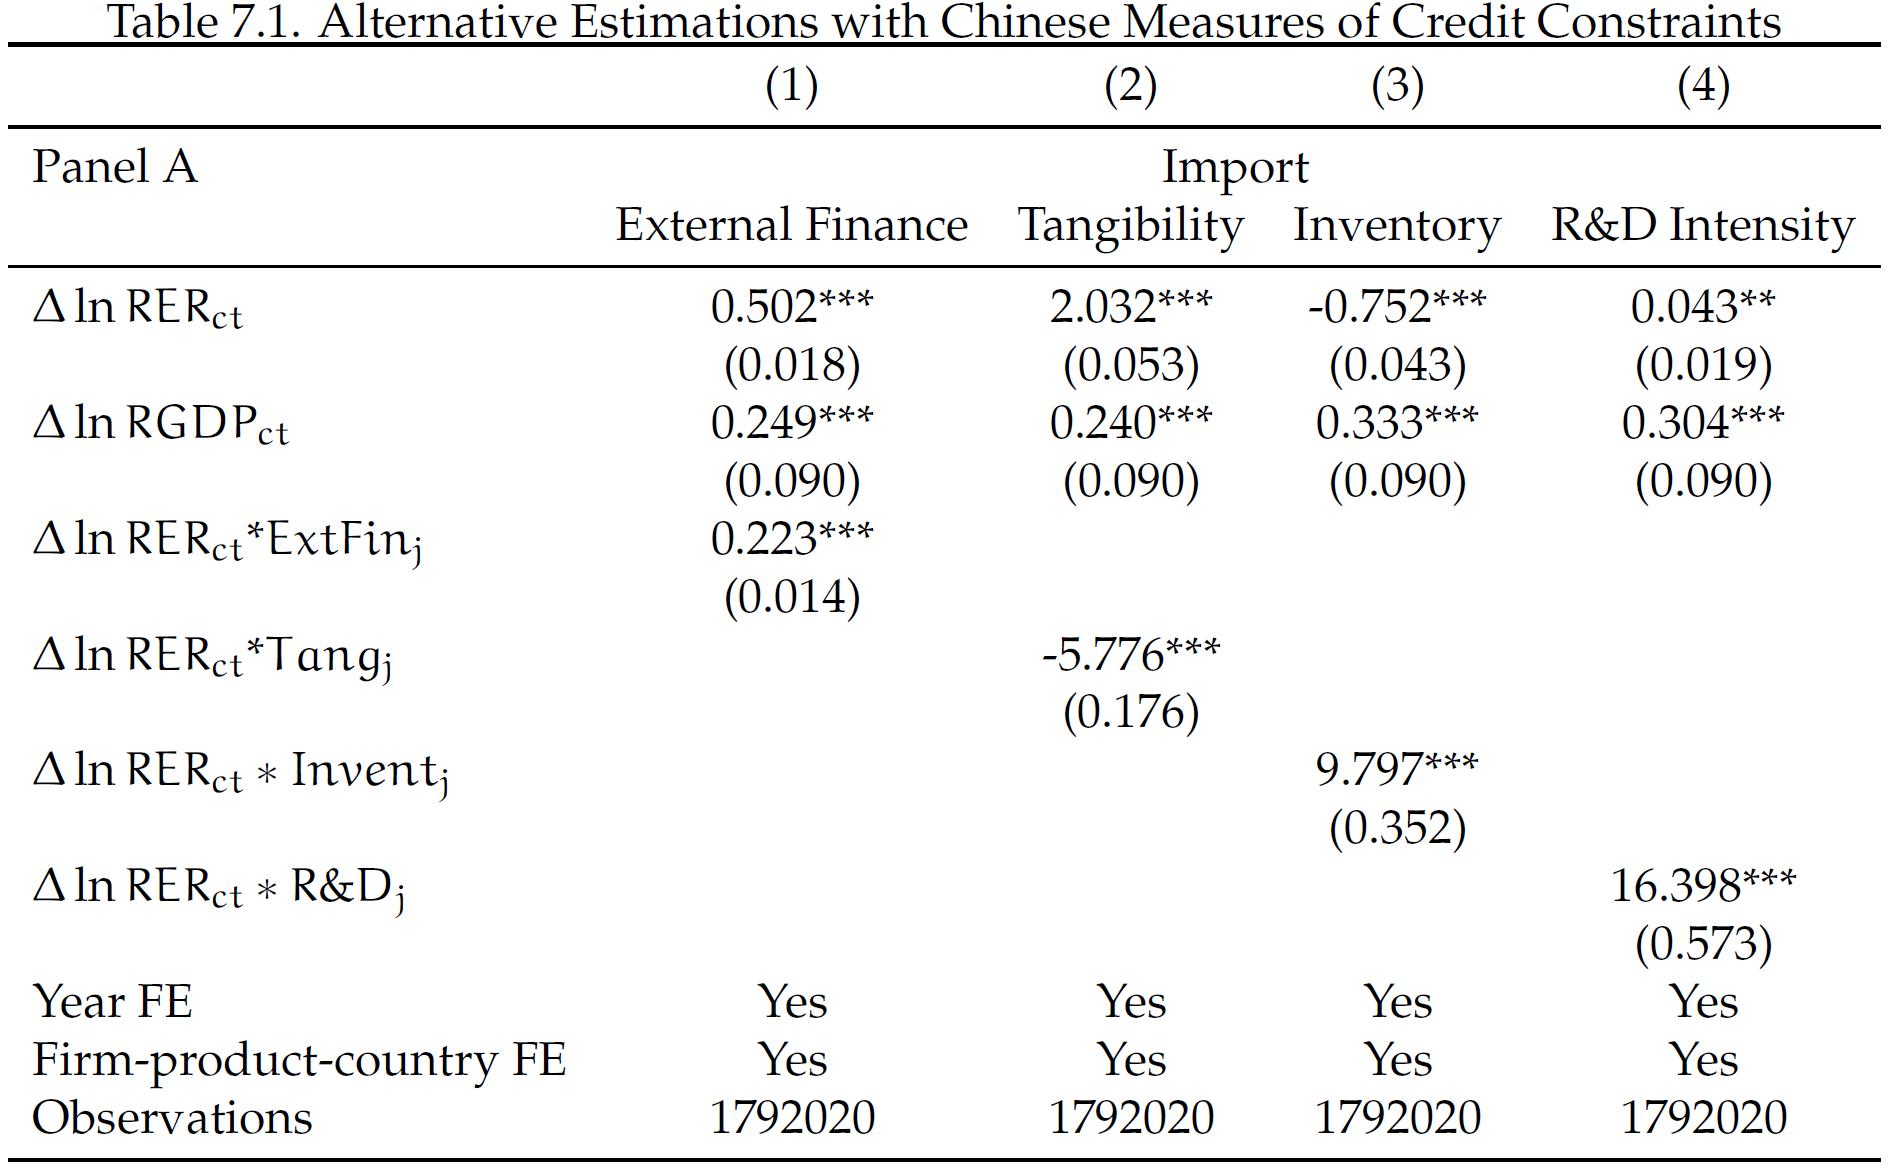
\includegraphics[width=0.9\columnwidth]{Table7.1A.jpg}
		\label{tab7.1A}
	\end{figure}
\end{frame}

\begin{frame}{Alternative Measures of Credit Constraints}
	\begin{figure}[htbp]
		\centering
		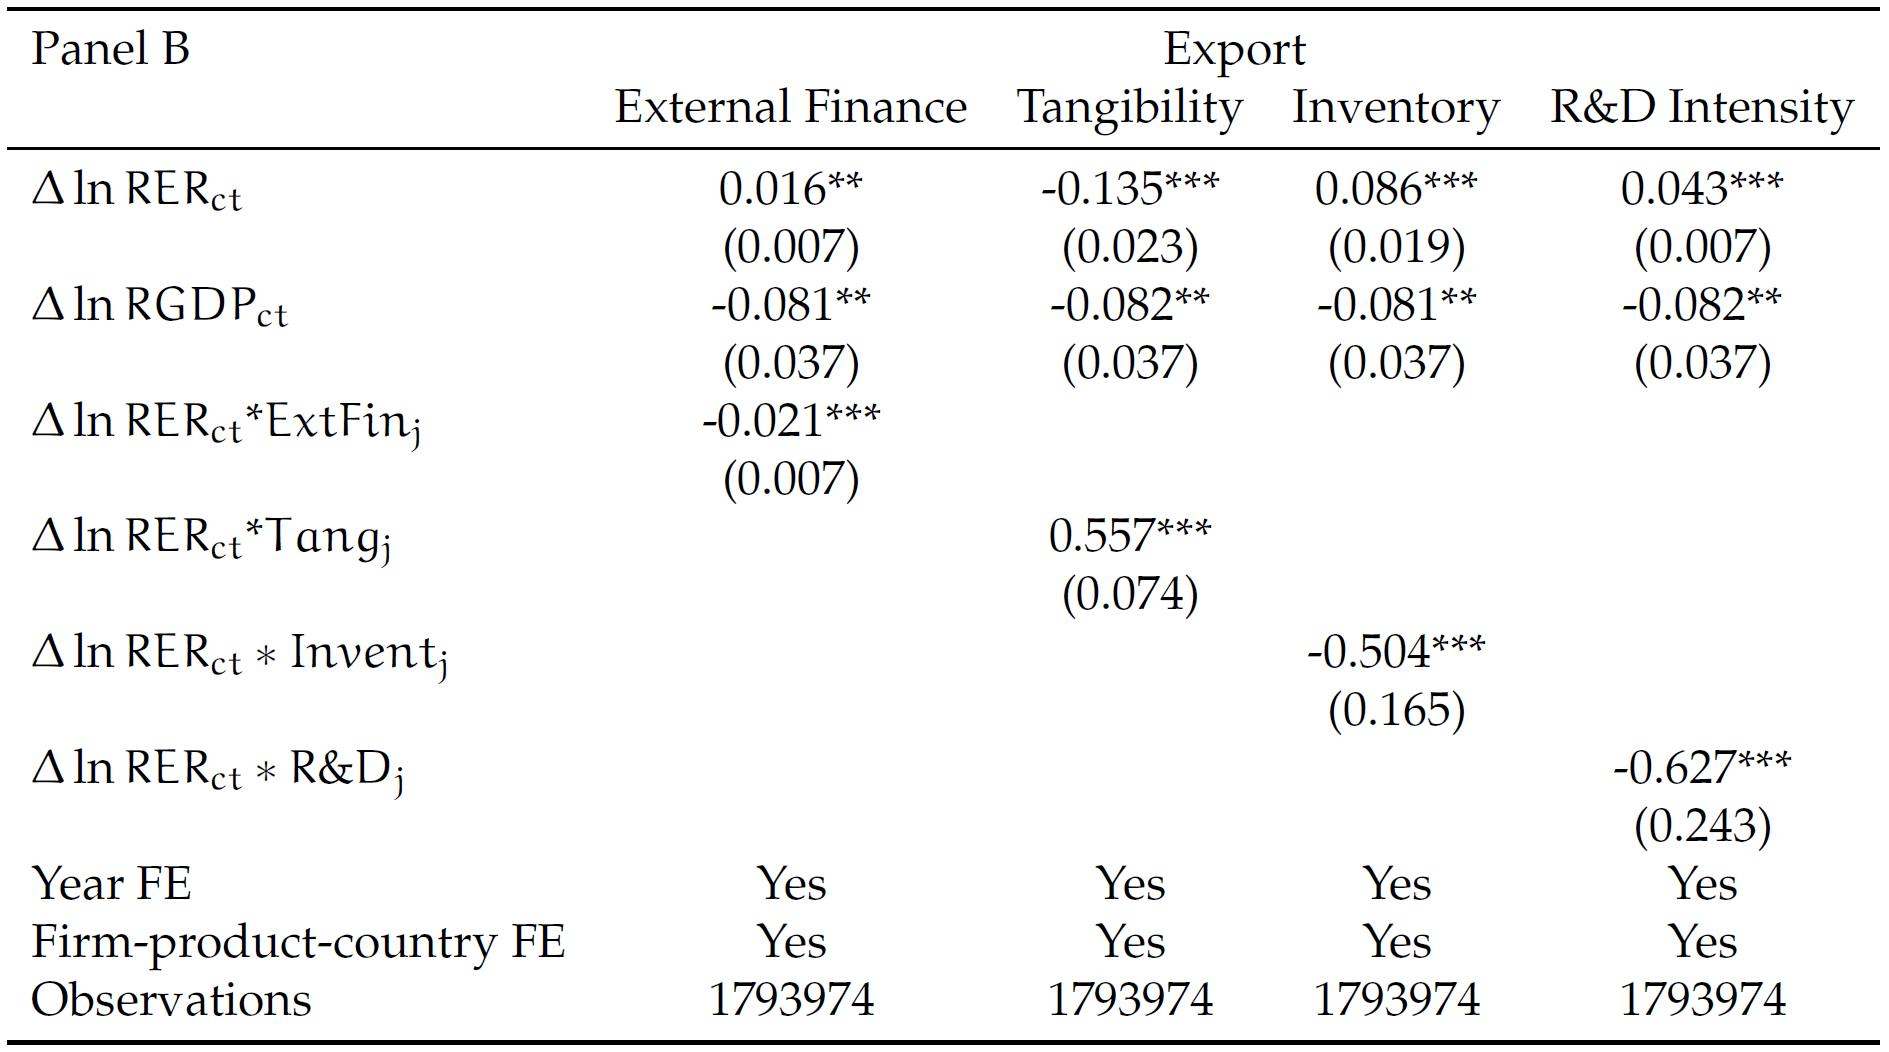
\includegraphics[width=0.9\columnwidth]{Table7.1B.jpg}
		\label{tab7.1B}
	\end{figure}
\end{frame}

\begin{frame}{Alternative Subsample: Two-way traders}
	\begin{itemize}
		\item Robustness check test 2: we use alternative sub-samples with only two-way traders who import and export at the same time.
	\end{itemize}
	\begin{figure}[htbp]
		\centering
		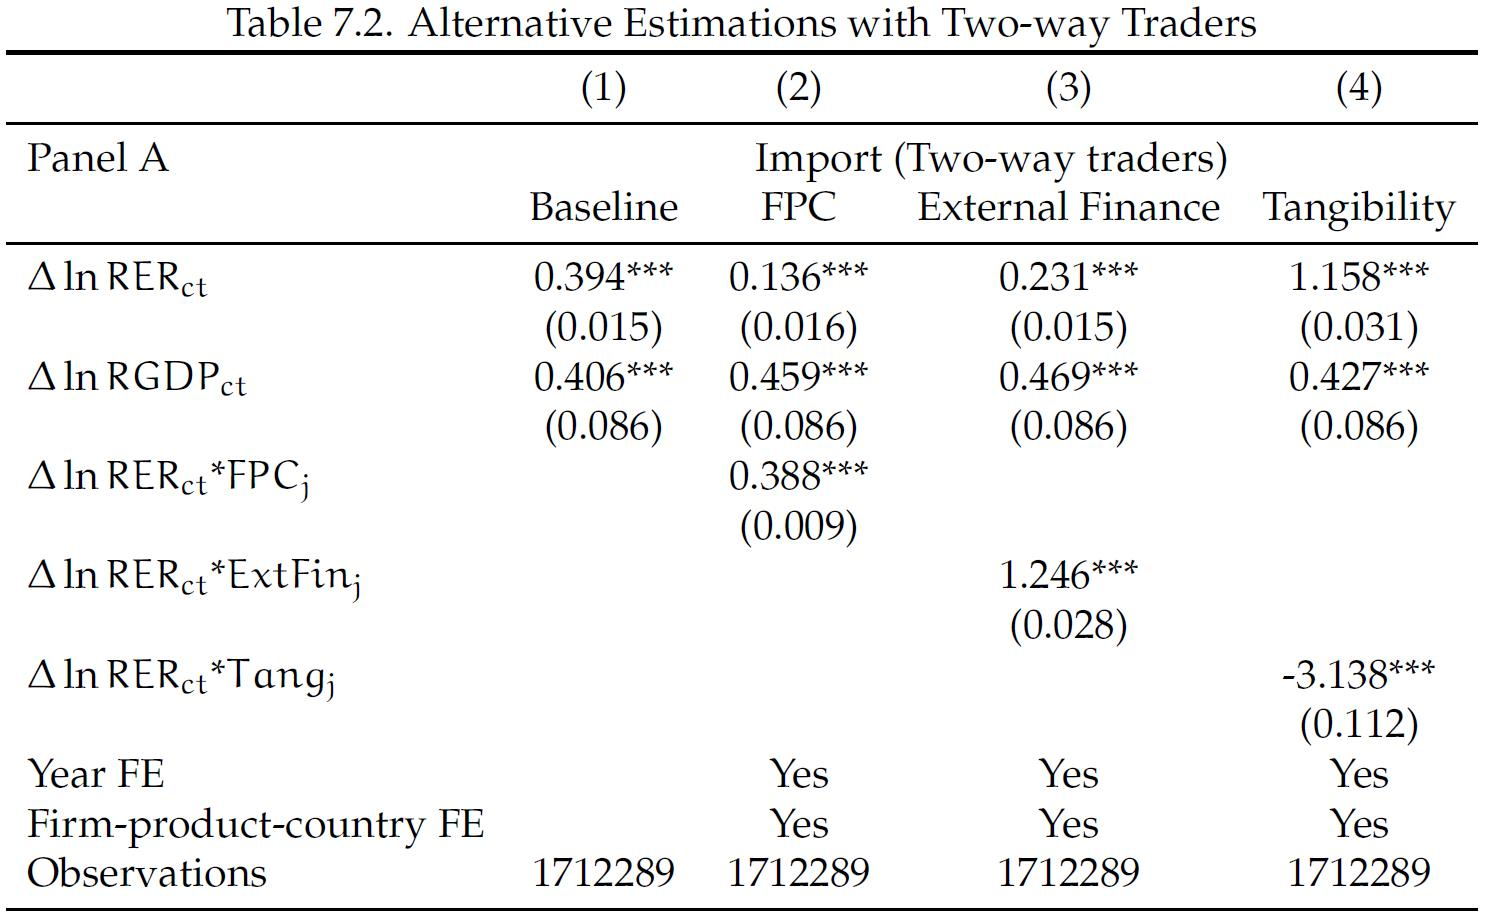
\includegraphics[width=0.85\columnwidth]{Table7.2A.jpg}
		\label{tab7.2A}
	\end{figure}
\end{frame}

\begin{frame}{Alternative Subsample: Two-way traders}
	\begin{figure}[htbp]
		\centering
		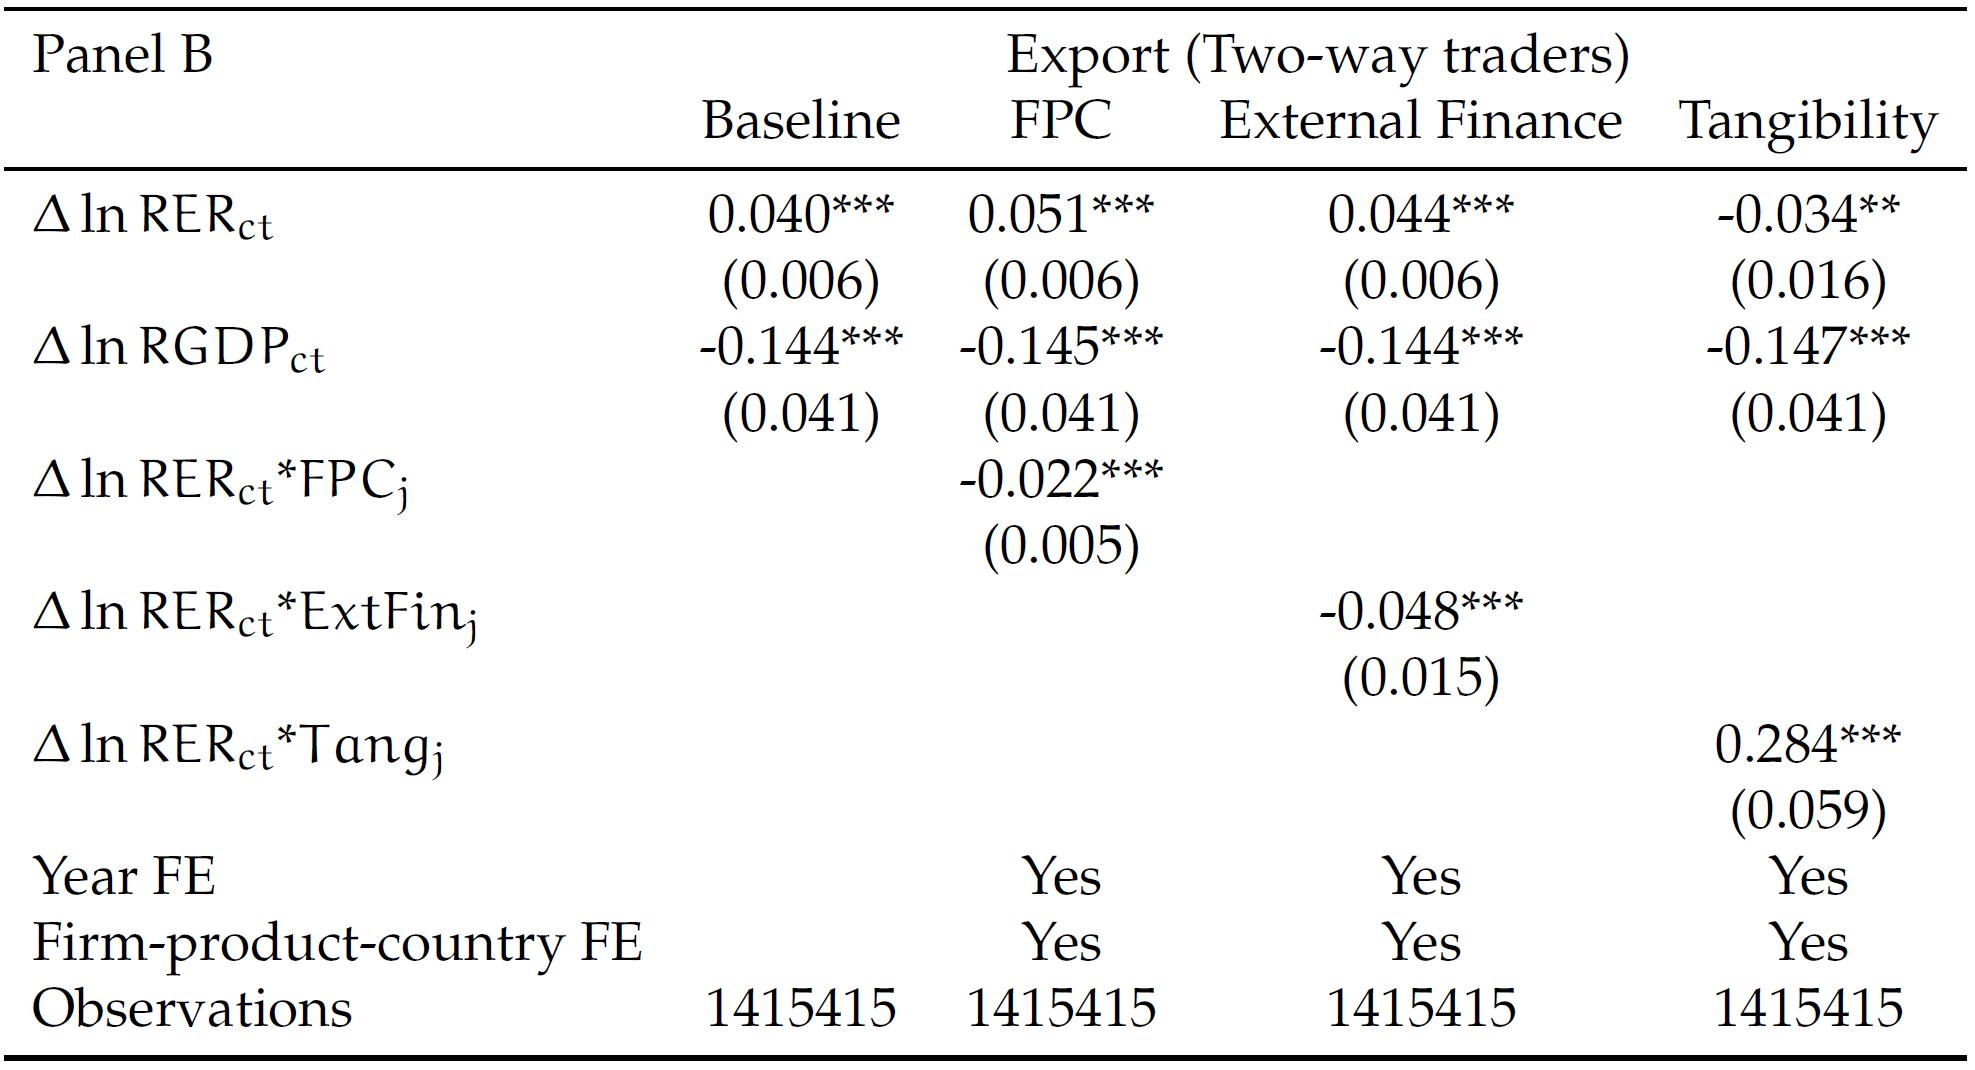
\includegraphics[width=0.85\columnwidth]{Table7.2B.jpg}
		\label{tab7.2B}
	\end{figure}
\end{frame}

\section{More Discussions}

\begin{frame}{Discussion on Firm Heterogeneity in Markup}
	\begin{itemize}
		\item Past literature suggest that different markup levels lead to
		heterogeneous export responses to exchange rate shocks.
	\end{itemize}
	\begin{figure}[htbp]
		\centering
		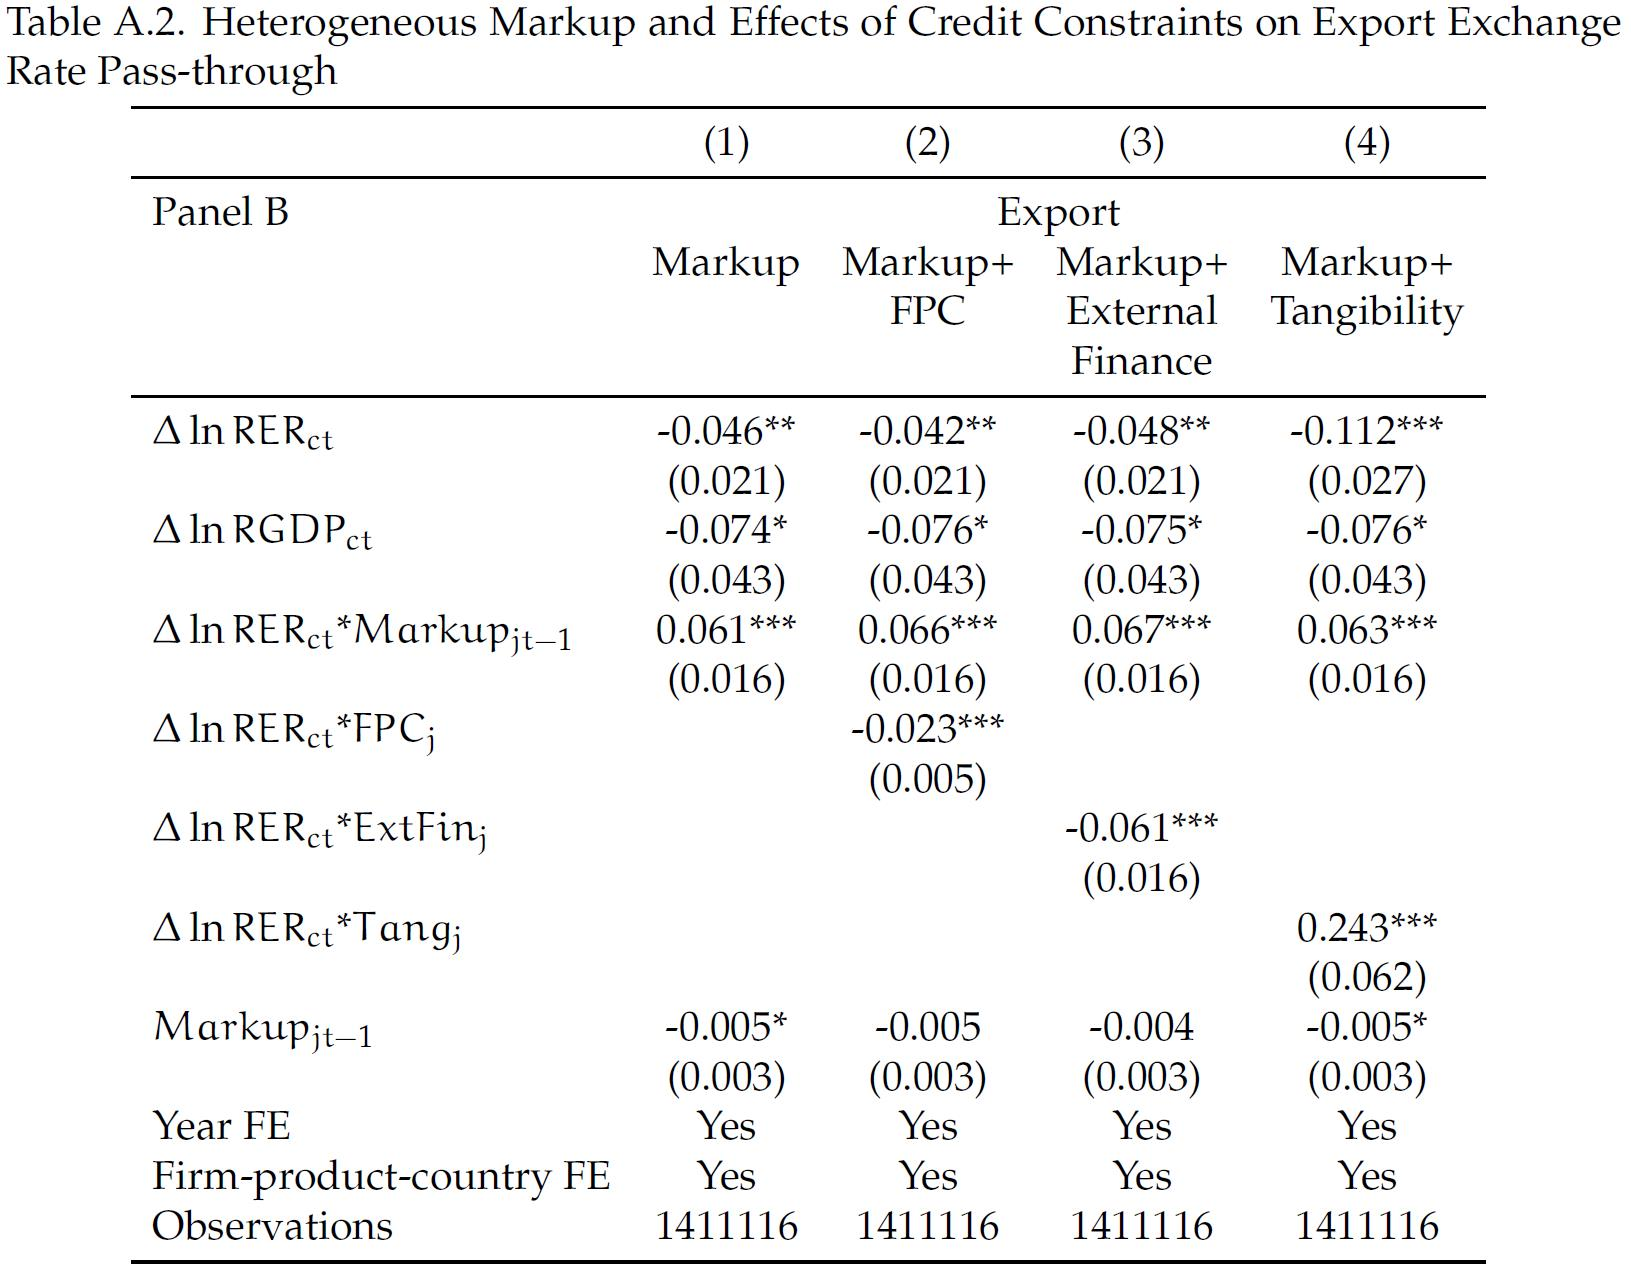
\includegraphics[width=0.75\columnwidth]{TableA2.jpg}
		\label{tabA2}
	\end{figure}
\end{frame}

\begin{frame}{Discussion on Firm Heterogeneity in Markup}
	\begin{itemize}
		\item Does this logic also work for import exchange rate pass-through?
		\item Do credit constraints still work after controlling for markup?
	\begin{figure}[htbp]
		\centering
		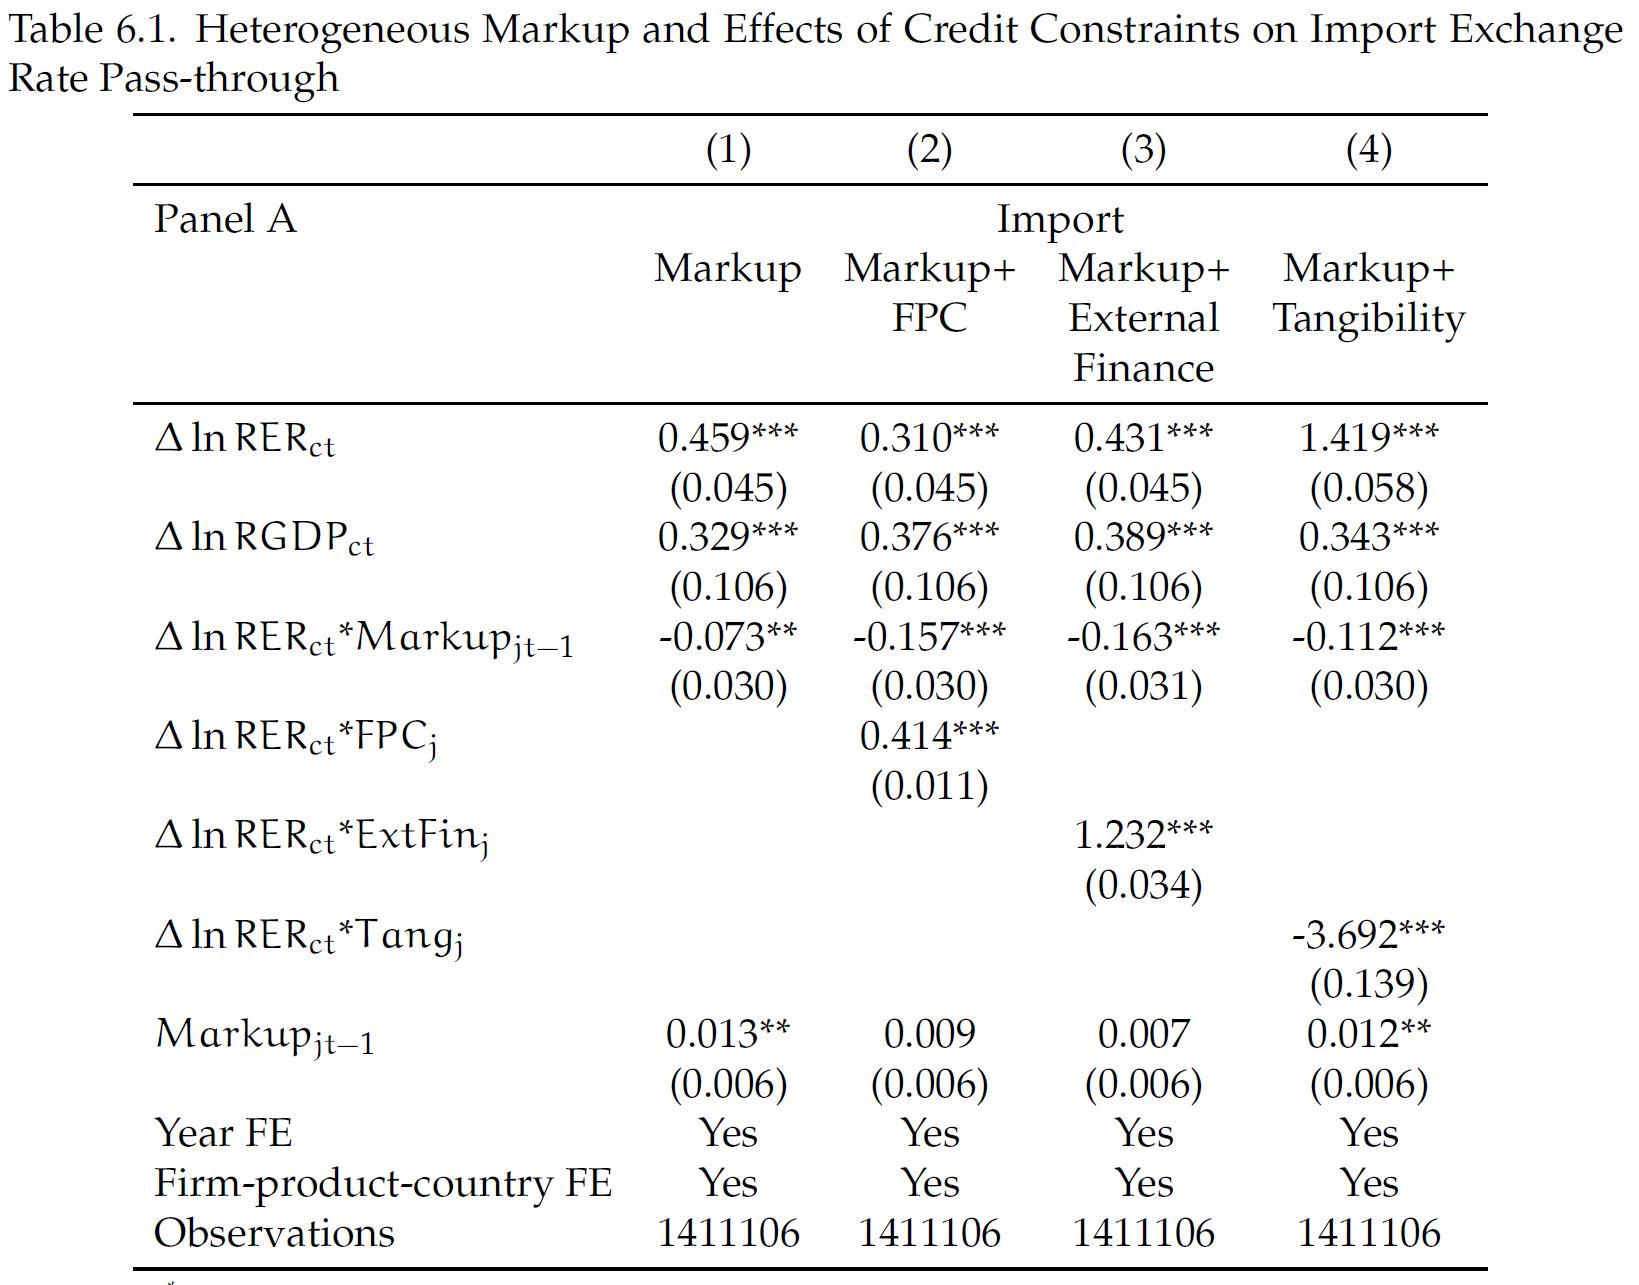
\includegraphics[width=0.75\columnwidth]{Table6.1.jpg}
		\label{tab6.1}
	\end{figure}
		
	\end{itemize}	
\end{frame}

\begin{frame}{Discussion on Firm Heterogeneity in Market Share}
	\begin{itemize}
		\item How a firm's market share affects its exchange rate pass-through?
	\end{itemize}
	\begin{figure}[htbp]
		\centering
		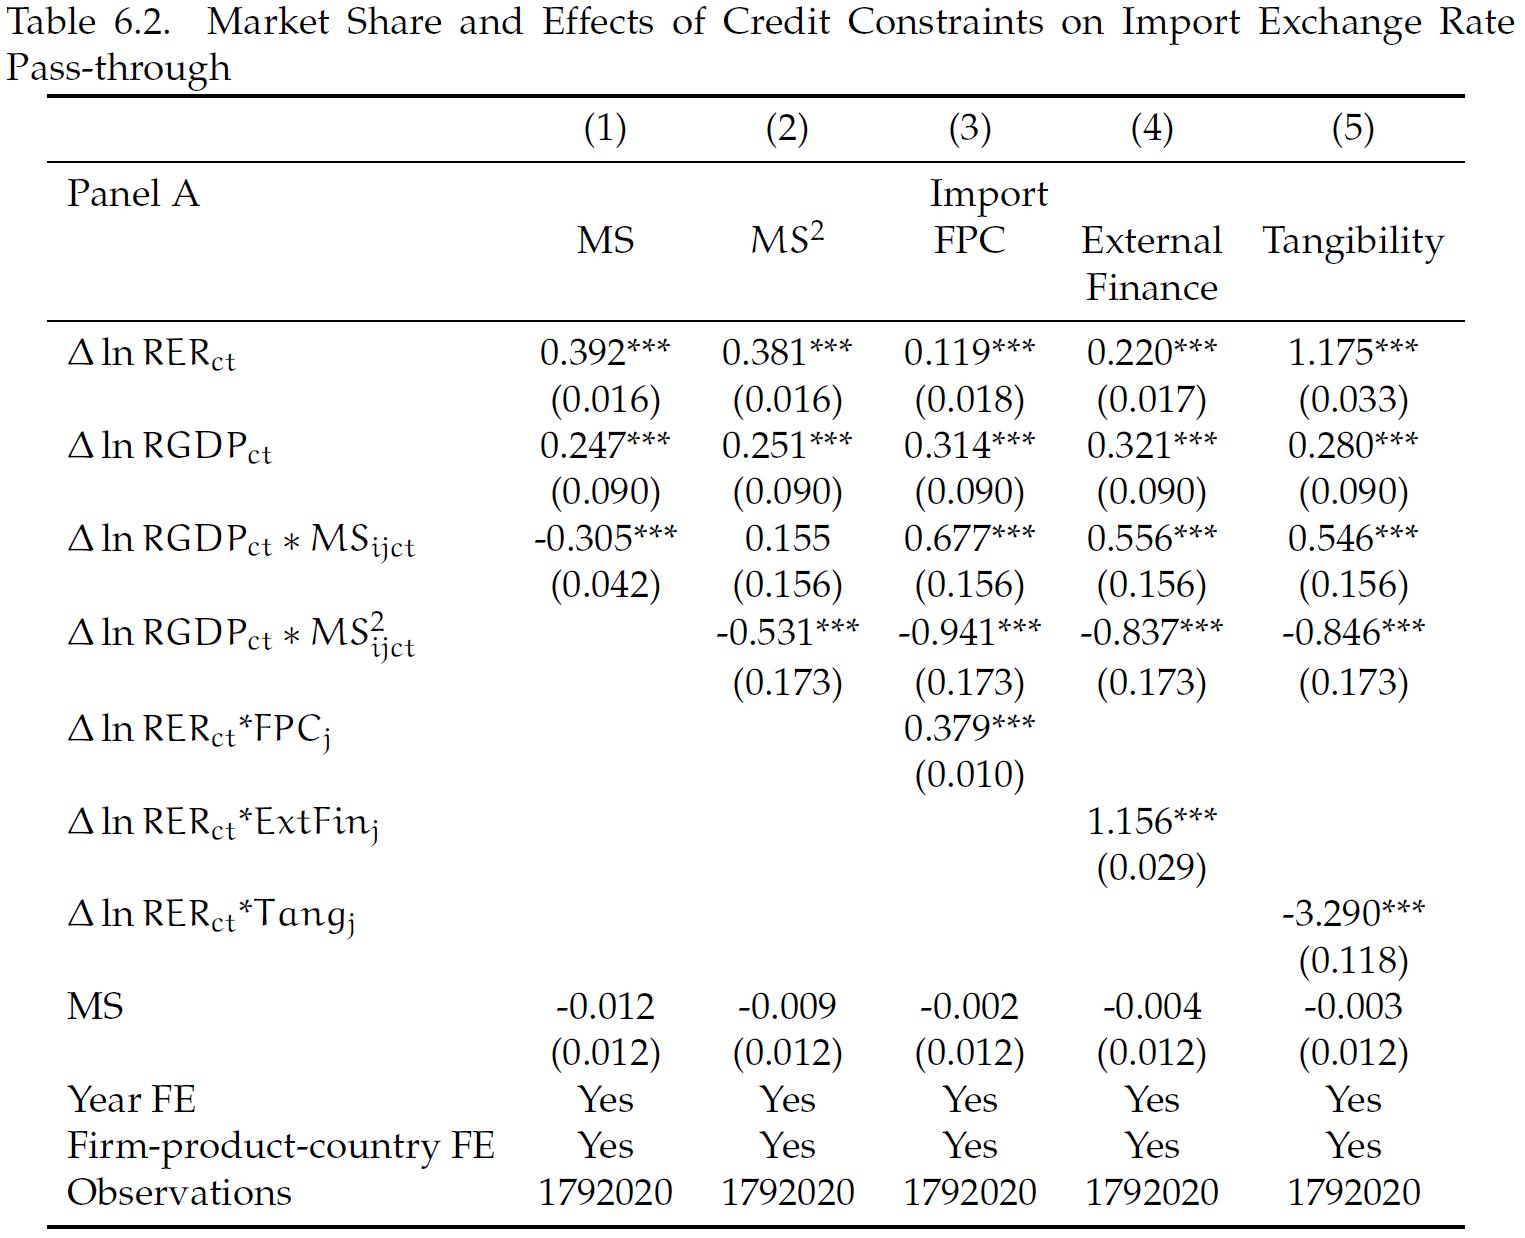
\includegraphics[width=0.8\columnwidth]{Table6.2.jpg}
		\label{tab6.2}
	\end{figure}
\end{frame}

\begin{frame}{Discussion on Firm Heterogeneity in Market Share}
	\begin{itemize}
		\item To test whether there is U-shape relationship between markup and ERPT, we perform group regressions by market share quartile.
	\end{itemize}
	\begin{figure}[htbp]
		\centering
		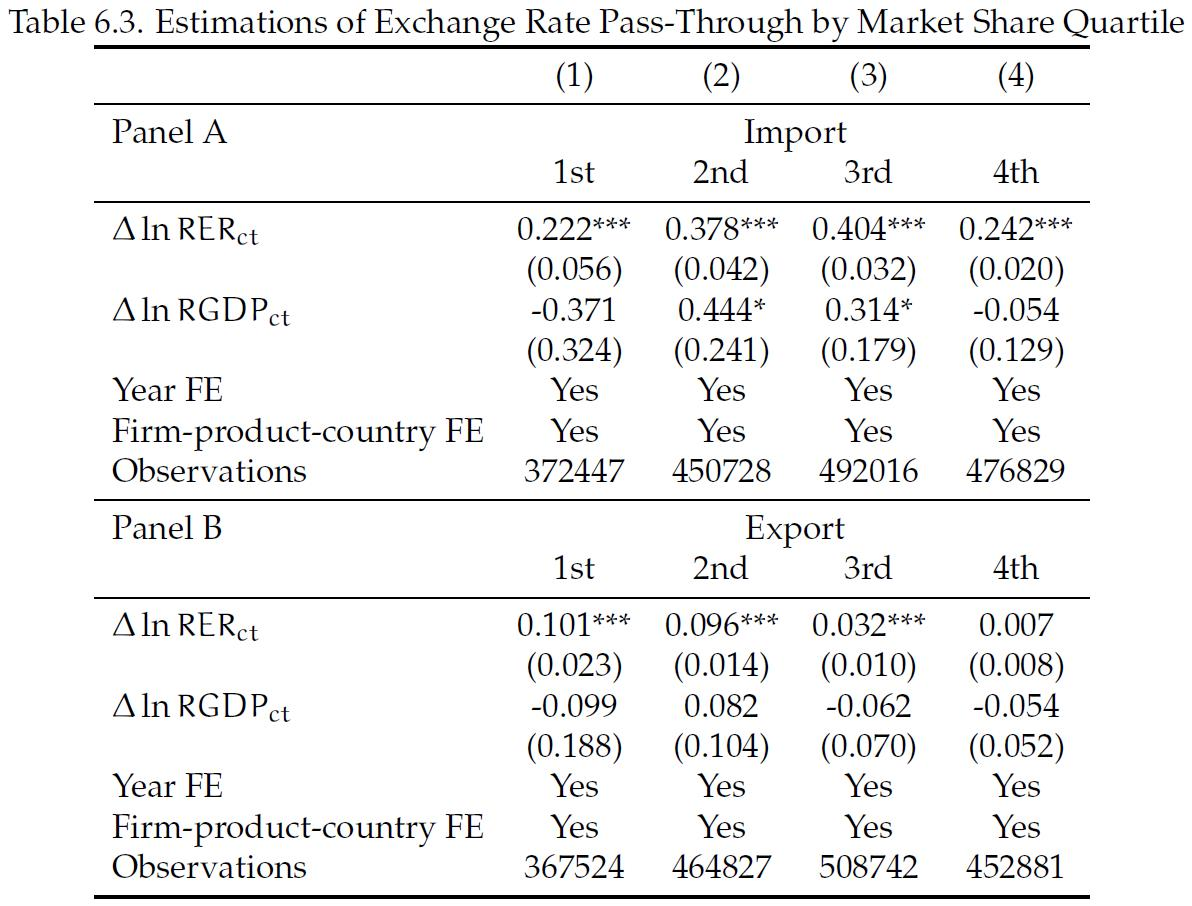
\includegraphics[width=0.8\columnwidth]{Table6.3.jpg}
		\label{tab6.3}
	\end{figure}
\end{frame}

\begin{frame}{Discussion on Future Research}
In what directions can we study the factors that determine exchange rate pass-through in the future?
	\begin{enumerate}
		\item Import-export Linkage
		\begin{itemize}
			\item "Pressure-reducing
			valve": when a firm has the ability to pass more exchange rate fluctuations to destination prices, it has more room to absorb price fluctuations of imported inputs.
			\item Advantages in some firm characteristics may bring
			greater bargaining power on both the import the export side and thus cause lower export and import price pass-through as in \cite{aik2014}.
		\end{itemize}
		\item Time Trend of China’s Exchange Rate Pass-through
		\begin{itemize}
			\item How do the (import and export) exchange rate pass-through levels of China evolve over time?
			\item Is this trend of exchange rate pass-through affected by loosening credit constraints and/or industry switching?
		\end{itemize}
	\end{enumerate}
\end{frame}

\section{Conclusion}

\begin{frame}{Conclusion}
	\begin{itemize}
		\item In this paper, we provide evidence at a disaggregated level for the incomplete import exchange rate pass-through in China and reveal how importers’ financial constraints affect the pass-through.
		\item We find that:
		\begin{enumerate}
			\item the average import exchange rate pass-through in China is around 35-40\%, far below the 95\% level for export pass-through;
			\item both import and export exchange rate pass-through are more complete for firms in industries with tighter credit constraints;
			\item import source diversity can effectively reduce import price pass-through and offset the effects of credit constraints
		\end{enumerate}
		\item In the future, we need to explore the underlying mechanism by which credit constraints affect exchange rate pass-through and the implications on the evolving trend of exchange rate pass-through. 
	\end{itemize}
\end{frame}

\begin{frame}{}
	\centering \Large
	\emph{Thank you! Questions Welcome!}
\end{frame}

\section*{Reference}

\begin{frame}[allowframebreaks]
	\frametitle{References}
	\bibliographystyle{apalike}
	\footnotesize
	\bibliography{ref.bib}
\end{frame}
	
\end{document}